\originalchapter{8.04 作业8：相干态、模型键与反射延迟}
来源为Spring 2016 Assignment 8, 2016年4月13日发布, 4月22日12时截止. 第1--5题中文转述与\textbf{AI独立解答}. 第5题保留Based on Griffiths 2.33、p.83署名, 按MIT提供的矩形障壁任务作通用宽度推导, 不补造未给的外书专用数据.
\originalsection{第1题：湮灭本征态与能量涨落}
\begin{exercise}
$\psi_\alpha=N\e^{\alpha a^\dagger}\varphi_0$, $\alpha$复. 求归一因子、湮灭本征值、能量均值与不确定度, 再由微分本征方程给归一位置波函数.
\end{exercise}
\begin{solution}
指数展开$\sum\alpha^n\ket n/\sqrt{n!}$, 范数平方$\e^{|\alpha|^2}$, 可取$N=\e^{-|\alpha|^2/2}$. $a\ket n=\sqrt n\ket{n-1}$移求和指标给$a\psi_\alpha=\alpha\psi_\alpha$. Poisson分布均值及方差$|\alpha|^2$, 所以$\langle H\rangle=\hbar\omega(|\alpha|^2+1/2)$,$\Delta H=\hbar\omega|\alpha|$.

位置表示$a=(x/d+d\partial_x)/\sqrt2$, $d=\sqrt{\hbar/(m\omega)}$, 一阶方程积分给$\psi=C\exp[-x^2/(2d^2)+\sqrt2\alpha x/d]$. 依题给Fock相位约定的归一常数为$C=(\pi d^2)^{-1/4}\exp[-\alpha^2/2-|\alpha|^2/2]$. 等价地令$x_0=\sqrt2d\operatorname{Re}\alpha,p_0=\sqrt2\hbar\operatorname{Im}\alpha/d$, 得$\psi=(\pi d^2)^{-1/4}\exp[-(x-x_0)^2/(2d^2)+\ii p_0(x-x_0/2)/\hbar]$. 常相位选取与题设位移一致.
\end{solution}
\originalsection{第2题：双点势与分子间距}
\begin{exercise}
双点势偶态方程$\xi=\lambda(1+\e^{-2\xi})$, $a_0=\hbar^2/(mg)$,$\lambda=a/a_0$,$E_\infty=mg^2/(2\hbar^2)>0$. 加原子间斥势$V_r(x)=\beta g/x$. (a)写电子能量并画其随$\lambda$变化及两端极限. (b)写$V_r(2a)$. (c)不同$\beta$画总能, $\beta=0.31$求稳定驻点.
\end{exercise}
\begin{solution}
电子能$E=-E_\infty(\xi/\lambda)^2=-E_\infty(1+\e^{-2\xi})^2$. $\lambda\to0$两点合成强度$2g$单点,$E\to-4E_\infty$; $\lambda\to\infty$则$E\to-E_\infty$. 斥能$\beta g/(2a)=\beta E_\infty/\lambda$, 总无量纲能$F=-(\xi/\lambda)^2+\beta/\lambda$. 正$\beta$时小距离$F\to+\infty$, 大距离$F\to-1$（从上方）, 较小$\beta$有中间极小与后续极大.

可用参数$\xi$避免超越隐式差分: $\lambda=\xi/(1+\e^{-2\xi})$, 对$F(\xi)$求导找零, 再以二阶导数判定. $\beta=.31$时稳定极小$\lambda=0.401295411652477$, $F=-1.02549451572266$; 还有$\lambda=1.80845855916$不稳定极大. 极小低于分离能$-1$, 才是本模型的稳定键, 与仅看负能量不同.
\begin{center}\begin{tikzpicture}
\begin{axis}[width=.82\textwidth,height=4.2cm,xlabel={$\lambda$},ylabel={$E/E_\infty$},grid=major,legend style={font=\small},ymin=-4.2,ymax=-.8]
\addplot+[mark=none] coordinates{(0.00504999833,-3.92118679) (0.0114900203,-3.82611315) (0.0180855027,-3.73450625) (0.024836223,-3.64622596) (0.0317418624,-3.56113825) (0.0388020069,-3.47911494) (0.0460161472,-3.40003342) (0.0533836806,-3.32377638) (0.0609039116,-3.2502316) (0.068576053,-3.17929168) (0.0763992279,-3.11085385) (0.0843724709,-3.04481977) (0.0924947299,-2.98109527) (0.100764868,-2.91959023) (0.109181666,-2.86021837) (0.117743823,-2.80289705) (0.126449962,-2.74754715) (0.135298627,-2.69409288) (0.144288292,-2.64246165) (0.153417357,-2.59258391) (0.162684158,-2.54439303) (0.172086962,-2.49782516) (0.181623975,-2.45281912) (0.191293345,-2.40931623) (0.201093162,-2.36726029) (0.211021463,-2.32659738) (0.221076234,-2.28727582) (0.231255417,-2.24924602) (0.241556906,-2.21246046) (0.251978557,-2.17687351) (0.262518188,-2.14244143) (0.273173581,-2.10912222) (0.283942488,-2.07687559) (0.294822634,-2.04566287) (0.305811717,-2.01544693) (0.316907415,-1.98619213) (0.328107385,-1.95786424) (0.33940927,-1.9304304) (0.3508107,-1.90385902) (0.362309294,-1.8781198) (0.373902666,-1.85318357) (0.385588424,-1.82902235) (0.397364174,-1.80560922) (0.409227526,-1.78291831) (0.421176092,-1.76092475) (0.433207488,-1.73960464) (0.445319343,-1.71893498) (0.457509294,-1.69889365) (0.469774991,-1.67945937) (0.482114101,-1.66061168) (0.494524307,-1.64233088) (0.507003312,-1.62459801) (0.519548841,-1.60739483) (0.532158638,-1.59070377) (0.544830477,-1.57450792) (0.557562154,-1.55879099) (0.570351495,-1.5435373) (0.583196353,-1.52873172) (0.596094614,-1.51435971) (0.609044192,-1.50040724) (0.622043036,-1.48686078) (0.635089129,-1.4737073) (0.648180486,-1.46093423) (0.66131516,-1.44852947) (0.674491238,-1.43648133) (0.687706845,-1.42477854) (0.700960143,-1.41341023) (0.714249332,-1.40236592) (0.72757265,-1.39163549) (0.740928373,-1.38120917) (0.754314818,-1.37107753) (0.767730339,-1.36123148) (0.781173331,-1.35166223) (0.794642226,-1.3423613) (0.808135499,-1.33332049) (0.821651661,-1.32453188) (0.835189265,-1.31598783) (0.848746901,-1.30768095) (0.8623232,-1.2996041) (0.875916831,-1.29175038) (0.889526501,-1.28411312) (0.903150956,-1.27668586) (0.916788981,-1.26946237) (0.930439395,-1.26243662) (0.944101059,-1.25560277) (0.957772867,-1.24895518) (0.97145375,-1.2424884) (0.985142677,-1.23619714) (0.998838648,-1.23007628) (1.0125407,-1.22412089) (1.02624791,-1.21832617) (1.03995937,-1.21268748) (1.05367424,-1.20720033) (1.06739166,-1.20186038) (1.08111086,-1.19666342) (1.09483105,-1.19160536) (1.10855151,-1.18668226) (1.12227153,-1.18189029) (1.13599043,-1.17722574) (1.14970755,-1.17268502) (1.16342229,-1.16826463) (1.17713403,-1.16396122) (1.19084223,-1.15977149) (1.20454633,-1.15569228) (1.21824582,-1.15172051) (1.2319402,-1.1478532) (1.24562901,-1.14408745) (1.25931181,-1.14042045) (1.27298816,-1.13684948) (1.28665767,-1.1333719) (1.30031997,-1.12998515) (1.31397468,-1.12668673) (1.32762148,-1.12347423) (1.34126004,-1.12034531) (1.35489006,-1.11729769) (1.36851126,-1.11432917) (1.38212338,-1.1114376) (1.39572617,-1.10862091) (1.4093194,-1.10587706) (1.42290285,-1.1032041) (1.43647633,-1.10060012) (1.45003964,-1.09806327) (1.46359263,-1.09559175) (1.47713513,-1.09318382) (1.49066699,-1.09083777) (1.5041881,-1.08855196) (1.51769832,-1.08632478) (1.53119757,-1.08415469) (1.54468573,-1.08204015) (1.55816273,-1.07997971) (1.57162849,-1.07797194) (1.58508296,-1.07601543) (1.59852607,-1.07410885) (1.61195779,-1.07225088) (1.62537808,-1.07044024) (1.6387869,-1.0686757) (1.65218426,-1.06695603) (1.66557013,-1.06528008) (1.6789445,-1.06364669) (1.6923074,-1.06205475) (1.70565882,-1.06050319) (1.71899878,-1.05899096) (1.73232731,-1.05751703) (1.74564444,-1.05608041) (1.75895019,-1.05468013) (1.77224462,-1.05331525) (1.78552777,-1.05198485) (1.79879969,-1.05068805) (1.81206042,-1.04942397) (1.82531004,-1.04819177) (1.8385486,-1.04699064) (1.85177617,-1.04581976) (1.86499282,-1.04467837) (1.87819863,-1.0435657) (1.89139366,-1.04248102) (1.90457801,-1.04142361) (1.91775175,-1.04039278) (1.93091497,-1.03938784) (1.94406776,-1.03840813) (1.9572102,-1.037453) (1.97034239,-1.03652184) (1.98346442,-1.03561402) (1.99657639,-1.03472895) (2.00967839,-1.03386606) (2.02277052,-1.03302478) (2.03585289,-1.03220456) (2.04892559,-1.03140486) (2.06198873,-1.03062517) (2.07504241,-1.02986498) (2.08808673,-1.02912378) (2.1011218,-1.02840111) (2.11414772,-1.02769649) (2.12716461,-1.02700947) (2.14017256,-1.02633959) (2.15317168,-1.02568644) (2.16616209,-1.02504957) (2.17914388,-1.0244286) (2.19211718,-1.0238231) (2.20508207,-1.0232327) (2.21803868,-1.02265701) (2.2309871,-1.02209566) (2.24392745,-1.02154829) (2.25685984,-1.02101455) (2.26978437,-1.0204941) (2.28270114,-1.0199866) (2.29561027,-1.01949173) (2.30851185,-1.01900916) (2.321406,-1.0185386) (2.33429282,-1.01807974) (2.34717241,-1.01763229) (2.36004488,-1.01719595) (2.37291033,-1.01677046) (2.38576886,-1.01635554) (2.39862058,-1.01595092) (2.41146558,-1.01555635) (2.42430397,-1.01517158) (2.43713584,-1.01479636) (2.44996129,-1.01443045) (2.46278043,-1.01407362) (2.47559334,-1.01372565) (2.48840012,-1.01338631) (2.50120088,-1.01305538) (2.5139957,-1.01273266) (2.52678467,-1.01241794) (2.53956789,-1.01211103) (2.55234545,-1.01181172) (2.56511745,-1.01151983) (2.57788396,-1.01123518) (2.59064508,-1.01095757) (2.6034009,-1.01068684) (2.6161515,-1.01042282) (2.62889697,-1.01016534) (2.64163739,-1.00991424) (2.65437284,-1.00966935) (2.66710342,-1.00943053) (2.67982919,-1.00919761) (2.69255025,-1.00897047) (2.70526666,-1.00874894) (2.71797852,-1.0085329) (2.73068589,-1.0083222) (2.74338885,-1.00811671) (2.75608748,-1.00791631) (2.76878185,-1.00772087) (2.78147204,-1.00753026) (2.79415811,-1.00734437) (2.80684014,-1.00716307) (2.81951821,-1.00698625) (2.83219237,-1.00681381) (2.8448627,-1.00664563) (2.85752926,-1.00648161) (2.87019213,-1.00632164) (2.88285136,-1.00616563) (2.89550702,-1.00601347) (2.90815918,-1.00586508) (2.9208079,-1.00572035) (2.93345323,-1.00557919) (2.94609524,-1.00544153) (2.958734,-1.00530727) (2.97136955,-1.00517632) (2.98400196,-1.00504861) (2.99663128,-1.00492405) (3.00925757,-1.00480257) (3.02188089,-1.00468409) (3.03450129,-1.00456854) (3.04711882,-1.00445584) (3.05973353,-1.00434592) (3.07234549,-1.00423872) (3.08495473,-1.00413416) (3.09756131,-1.00403219) (3.11016528,-1.00393273) (3.12276669,-1.00383573) (3.13536558,-1.00374113) (3.147962,-1.00364886) (3.160556,-1.00355886) (3.17314763,-1.00347109) (3.18573692,-1.00338549) (3.19832393,-1.003302) (3.21090869,-1.00322056) (3.22349125,-1.00314114) (3.23607164,-1.00306368) (3.24864992,-1.00298813) (3.26122612,-1.00291445) (3.27380028,-1.00284258) (3.28637244,-1.00277249) (3.29894264,-1.00270412) (3.31151091,-1.00263745) (3.32407729,-1.00257241) (3.33664183,-1.00250899) (3.34920454,-1.00244712) (3.36176548,-1.00238679) (3.37432467,-1.00232794) (3.38688215,-1.00227054) (3.39943794,-1.00221456) (3.4119921,-1.00215996) (3.42454463,-1.00210671) (3.43709559,-1.00205477) (3.44964499,-1.00200412) (3.46219286,-1.00195471) (3.47473925,-1.00190652) (3.48728417,-1.00185952) (3.49982766,-1.00181368) (3.51236974,-1.00176896) (3.52491045,-1.00172536) (3.5374498,-1.00168282) (3.54998783,-1.00164134) (3.56252456,-1.00160088) (3.57506001,-1.00156142) (3.58759422,-1.00152293) (3.60012721,-1.00148538) (3.61265899,-1.00144877) (3.6251896,-1.00141306) (3.63771906,-1.00137823) (3.6502474,-1.00134425) (3.66277462,-1.00131112) (3.67530076,-1.0012788) (3.68782584,-1.00124728) (3.70034988,-1.00121653) (3.7128729,-1.00118655) (3.72539492,-1.0011573) (3.73791596,-1.00112878) (3.75043604,-1.00110095) (3.76295518,-1.00107382) (3.77547339,-1.00104735) (3.78799071,-1.00102154) (3.80050714,-1.00099636) (3.8130227,-1.0009718) (3.82553741,-1.00094785) (3.8380513,-1.00092449) (3.85056436,-1.0009017) (3.86307663,-1.00087948) (3.87558811,-1.0008578) (3.88809883,-1.00083666) (3.9006088,-1.00081604) (3.91311803,-1.00079593) (3.92562654,-1.00077631) (3.93813435,-1.00075718) (3.95064146,-1.00073852) (3.9631479,-1.00072031) (3.97565367,-1.00070256) (3.9881588,-1.00068525) (4.00066328,-1.00066836) (4.01316715,-1.00065189) (4.0256704,-1.00063582) (4.03817306,-1.00062015) (4.05067512,-1.00060487) (4.06317662,-1.00058996) (4.07567755,-1.00057542) (4.08817794,-1.00056124) (4.10067778,-1.00054741) (4.1131771,-1.00053392) (4.1256759,-1.00052076) (4.13817419,-1.00050793) (4.15067199,-1.00049541) (4.1631693,-1.0004832) (4.17566614,-1.00047129) (4.18816251,-1.00045968) (4.20065843,-1.00044835) (4.2131539,-1.0004373) (4.22564893,-1.00042652) (4.23814353,-1.00041601) (4.25063772,-1.00040576) (4.2631315,-1.00039576) (4.27562487,-1.00038601) (4.28811785,-1.00037649) (4.30061045,-1.00036722) (4.31310267,-1.00035817) (4.32559451,-1.00034934) (4.338086,-1.00034073) (4.35057714,-1.00033233) (4.36306793,-1.00032414) (4.37555837,-1.00031616) (4.38804849,-1.00030837) (4.40053828,-1.00030077) (4.41302776,-1.00029335) (4.42551692,-1.00028613) (4.43800578,-1.00027907) (4.45049434,-1.0002722) (4.4629826,-1.00026549) (4.47547058,-1.00025895) (4.48795828,-1.00025257) (4.50044571,-1.00024634) (4.51293287,-1.00024027) (4.52541976,-1.00023435) (4.5379064,-1.00022858) (4.55039279,-1.00022294) (4.56287893,-1.00021745) (4.57536483,-1.00021209) (4.58785049,-1.00020686) (4.60033593,-1.00020177) (4.61282113,-1.00019679) (4.62530612,-1.00019194) (4.63779089,-1.00018721) (4.65027545,-1.0001826) (4.6627598,-1.0001781) (4.67524394,-1.00017371) (4.68772789,-1.00016943) (4.70021165,-1.00016526) (4.71269521,-1.00016118) (4.72517859,-1.00015721) (4.73766178,-1.00015334) (4.7501448,-1.00014956) (4.76262764,-1.00014587) (4.77511031,-1.00014228) (4.78759282,-1.00013877) (4.80007516,-1.00013535) (4.81255734,-1.00013202) (4.82503936,-1.00012877) (4.83752123,-1.00012559) (4.85000295,-1.0001225) (4.86248453,-1.00011948) (4.87496596,-1.00011653) (4.88744725,-1.00011366) (4.8999284,-1.00011086) (4.91240942,-1.00010813) (4.9248903,-1.00010547) (4.93737106,-1.00010287) (4.94985169,-1.00010033) (4.9623322,-1.00009786) (4.97481259,-1.00009545) (4.98729286,-1.0000931) (4.99977301,-1.0000908)};
\addlegendentry{电子能}
\end{axis}\end{tikzpicture}\end{center}
\begin{center}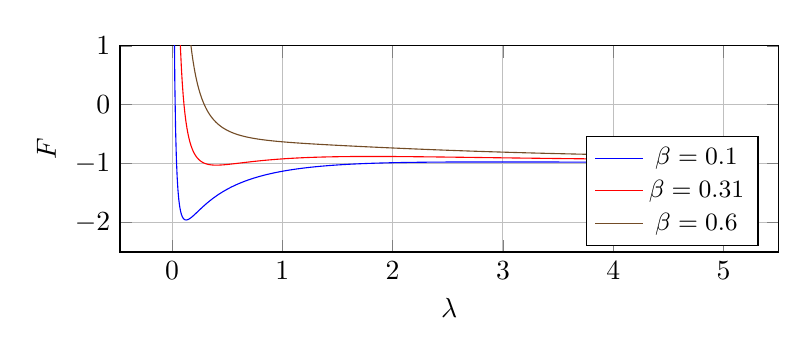
\begin{tikzpicture}
\begin{axis}[width=.82\textwidth,height=4.2cm,xlabel={$\lambda$},ylabel={$F$},grid=major,legend style={font=\small},ymin=-2.5,ymax=1,legend pos=south east]
\addplot+[mark=none] coordinates{(0.00504999833,15.8807999) (0.0114900203,4.87709167) (0.0180855027,1.79478435) (0.024836223,0.380151163) (0.0317418624,-0.410724498) (0.0388020069,-0.901928657) (0.0460161472,-1.22688321) (0.0533836806,-1.45054473) (0.0609039116,-1.60830093) (0.068576053,-1.72105668) (0.0763992279,-1.8019401) (0.0843724709,-1.85959905) (0.0924947299,-1.89995259) (0.100764868,-1.92718086) (0.109181666,-1.94431368) (0.117743823,-1.9535956) (0.126449962,-1.95672049) (0.135298627,-1.95498708) (0.144288292,-1.94940472) (0.153417357,-1.94076718) (0.162684158,-1.92970503) (0.172086962,-1.91672362) (0.181623975,-1.90223101) (0.191293345,-1.8865589) (0.201093162,-1.86997834) (0.211021463,-1.85271194) (0.221076234,-1.83494316) (0.231255417,-1.81682372) (0.241556906,-1.79847933) (0.251978557,-1.78001435) (0.262518188,-1.76151544) (0.273173581,-1.74305461) (0.283942488,-1.7246916) (0.294822634,-1.70647589) (0.305811717,-1.68844834) (0.316907415,-1.67064256) (0.328107385,-1.65308598) (0.33940927,-1.63580085) (0.3508107,-1.61880501) (0.362309294,-1.60211252) (0.373902666,-1.58573429) (0.385588424,-1.56967846) (0.397364174,-1.5539509) (0.409227526,-1.53855547) (0.421176092,-1.52349437) (0.433207488,-1.50876837) (0.445319343,-1.49437703) (0.457509294,-1.48031885) (0.469774991,-1.4665915) (0.482114101,-1.4531919) (0.494524307,-1.44011635) (0.507003312,-1.42736064) (0.519548841,-1.41492014) (0.532158638,-1.40278988) (0.544830477,-1.39096459) (0.557562154,-1.37943879) (0.570351495,-1.36820682) (0.583196353,-1.35726289) (0.596094614,-1.34660111) (0.609044192,-1.33621554) (0.622043036,-1.3261002) (0.635089129,-1.31624908) (0.648180486,-1.30665621) (0.66131516,-1.29731564) (0.674491238,-1.28822143) (0.687706845,-1.27936774) (0.700960143,-1.27074877) (0.714249332,-1.26235879) (0.72757265,-1.25419217) (0.740928373,-1.24624335) (0.754314818,-1.23850689) (0.767730339,-1.23097741) (0.781173331,-1.22364967) (0.794642226,-1.2165185) (0.808135499,-1.20957886) (0.821651661,-1.2028258) (0.835189265,-1.19625449) (0.848746901,-1.1898602) (0.8623232,-1.1836383) (0.875916831,-1.17758429) (0.889526501,-1.17169376) (0.903150956,-1.1659624) (0.916788981,-1.16038601) (0.930439395,-1.15496051) (0.944101059,-1.1496819) (0.957772867,-1.1445463) (0.97145375,-1.13954989) (0.985142677,-1.134689) (0.998838648,-1.12996001) (1.0125407,-1.12535943) (1.02624791,-1.12088382) (1.03995937,-1.11652987) (1.05367424,-1.11229434) (1.06739166,-1.10817406) (1.08111086,-1.10416596) (1.09483105,-1.10026707) (1.10855151,-1.09647446) (1.12227153,-1.0927853) (1.13599043,-1.08919683) (1.14970755,-1.08570638) (1.16342229,-1.08231132) (1.17713403,-1.07900912) (1.19084223,-1.07579731) (1.20454633,-1.07267348) (1.21824582,-1.06963527) (1.2319402,-1.06668043) (1.24562901,-1.06380673) (1.25931181,-1.061012) (1.27298816,-1.05829416) (1.28665767,-1.05565115) (1.30031997,-1.053081) (1.31397468,-1.05058176) (1.32762148,-1.04815155) (1.34126004,-1.04578855) (1.35489006,-1.04349097) (1.36851126,-1.04125707) (1.38212338,-1.03908516) (1.39572617,-1.03697362) (1.4093194,-1.03492082) (1.42290285,-1.03292523) (1.43647633,-1.03098533) (1.45003964,-1.02909964) (1.46359263,-1.02726673) (1.47713513,-1.02548521) (1.49066699,-1.02375371) (1.5041881,-1.02207091) (1.51769832,-1.02043554) (1.53119757,-1.01884633) (1.54468573,-1.01730207) (1.55816273,-1.01580156) (1.57162849,-1.01434367) (1.58508296,-1.01292725) (1.59852607,-1.01155123) (1.61195779,-1.01021452) (1.62537808,-1.0089161) (1.6387869,-1.00765495) (1.65218426,-1.00643009) (1.66557013,-1.00524057) (1.6789445,-1.00408546) (1.6923074,-1.00296383) (1.70565882,-1.00187482) (1.71899878,-1.00081756) (1.73232731,-0.999791221) (1.74564444,-0.998794977) (1.75895019,-0.997828038) (1.77224462,-0.996889631) (1.78552777,-0.995979004) (1.79879969,-0.995095422) (1.81206042,-0.994238173) (1.82531004,-0.99340656) (1.8385486,-0.992599906) (1.85177617,-0.991817553) (1.86499282,-0.991058858) (1.87819863,-0.990323195) (1.89139366,-0.989609955) (1.90457801,-0.988918545) (1.91775175,-0.988248387) (1.93091497,-0.987598918) (1.94406776,-0.98696959) (1.9572102,-0.98635987) (1.97034239,-0.985769236) (1.98346442,-0.985197183) (1.99657639,-0.984643217) (2.00967839,-0.984106858) (2.02277052,-0.983587637) (2.03585289,-0.983085098) (2.04892559,-0.982598797) (2.06198873,-0.982128302) (2.07504241,-0.981673191) (2.08808673,-0.981233053) (2.1011218,-0.980807488) (2.11414772,-0.980396107) (2.12716461,-0.979998531) (2.14017256,-0.979614389) (2.15317168,-0.979243321) (2.16616209,-0.978884977) (2.17914388,-0.978539015) (2.19211718,-0.978205101) (2.20508207,-0.977882912) (2.21803868,-0.977572131) (2.2309871,-0.97727245) (2.24392745,-0.976983571) (2.25685984,-0.976705199) (2.26978437,-0.976437052) (2.28270114,-0.976178851) (2.29561027,-0.975930326) (2.30851185,-0.975691215) (2.321406,-0.975461261) (2.33429282,-0.975240215) (2.34717241,-0.975027832) (2.36004488,-0.974823876) (2.37291033,-0.974628117) (2.38576886,-0.974440328) (2.39862058,-0.974260292) (2.41146558,-0.974087794) (2.42430397,-0.973922627) (2.43713584,-0.973764589) (2.44996129,-0.973613481) (2.46278043,-0.973469111) (2.47559334,-0.973331293) (2.48840012,-0.973199844) (2.50120088,-0.973074587) (2.5139957,-0.972955347) (2.52678467,-0.972841957) (2.53956789,-0.972734252) (2.55234545,-0.972632072) (2.56511745,-0.972535262) (2.57788396,-0.97244367) (2.59064508,-0.972357147) (2.6034009,-0.97227555) (2.6161515,-0.972198738) (2.62889697,-0.972126575) (2.64163739,-0.972058928) (2.65437284,-0.971995667) (2.66710342,-0.971936666) (2.67982919,-0.971881802) (2.69255025,-0.971830954) (2.70526666,-0.971784007) (2.71797852,-0.971740847) (2.73068589,-0.971701363) (2.74338885,-0.971665448) (2.75608748,-0.971632995) (2.76878185,-0.971603904) (2.78147204,-0.971578075) (2.79415811,-0.971555411) (2.80684014,-0.971535817) (2.81951821,-0.971519201) (2.83219237,-0.971505475) (2.8448627,-0.97149455) (2.85752926,-0.971486343) (2.87019213,-0.97148077) (2.88285136,-0.971477751) (2.89550702,-0.971477207) (2.90815918,-0.971479063) (2.9208079,-0.971483244) (2.93345323,-0.971489678) (2.94609524,-0.971498295) (2.958734,-0.971509026) (2.97136955,-0.971521804) (2.98400196,-0.971536564) (2.99663128,-0.971553244) (3.00925757,-0.971571781) (3.02188089,-0.971592116) (3.03450129,-0.971614191) (3.04711882,-0.971637949) (3.05973353,-0.971663334) (3.07234549,-0.971690293) (3.08495473,-0.971718774) (3.09756131,-0.971748726) (3.11016528,-0.971780099) (3.12276669,-0.971812845) (3.13536558,-0.971846918) (3.147962,-0.971882271) (3.160556,-0.97191886) (3.17314763,-0.971956642) (3.18573692,-0.971995575) (3.19832393,-0.972035619) (3.21090869,-0.972076733) (3.22349125,-0.972118878) (3.23607164,-0.972162018) (3.24864992,-0.972206115) (3.26122612,-0.972251134) (3.27380028,-0.97229704) (3.28637244,-0.9723438) (3.29894264,-0.972391381) (3.31151091,-0.97243975) (3.32407729,-0.972488878) (3.33664183,-0.972538734) (3.34920454,-0.972589289) (3.36176548,-0.972640513) (3.37432467,-0.972692381) (3.38688215,-0.972744864) (3.39943794,-0.972797937) (3.4119921,-0.972851574) (3.42454463,-0.97290575) (3.43709559,-0.972960442) (3.44964499,-0.973015626) (3.46219286,-0.973071279) (3.47473925,-0.973127381) (3.48728417,-0.973183908) (3.49982766,-0.97324084) (3.51236974,-0.973298158) (3.52491045,-0.973355841) (3.5374498,-0.973413871) (3.54998783,-0.973472229) (3.56252456,-0.973530896) (3.57506001,-0.973589857) (3.58759422,-0.973649093) (3.60012721,-0.973708588) (3.61265899,-0.973768327) (3.6251896,-0.973828293) (3.63771906,-0.973888472) (3.6502474,-0.973948849) (3.66277462,-0.974009411) (3.67530076,-0.974070142) (3.68782584,-0.974131031) (3.70034988,-0.974192063) (3.7128729,-0.974253227) (3.72539492,-0.974314511) (3.73791596,-0.974375901) (3.75043604,-0.974437388) (3.76295518,-0.97449896) (3.77547339,-0.974560606) (3.78799071,-0.974622316) (3.80050714,-0.97468408) (3.8130227,-0.974745888) (3.82553741,-0.97480773) (3.8380513,-0.974869598) (3.85056436,-0.974931482) (3.86307663,-0.974993374) (3.87558811,-0.975055265) (3.88809883,-0.975117148) (3.9006088,-0.975179015) (3.91311803,-0.975240858) (3.92562654,-0.975302669) (3.93813435,-0.975364442) (3.95064146,-0.975426171) (3.9631479,-0.975487847) (3.97565367,-0.975549465) (3.9881588,-0.97561102) (4.00066328,-0.975672503) (4.01316715,-0.975733911) (4.0256704,-0.975795238) (4.03817306,-0.975856477) (4.05067512,-0.975917624) (4.06317662,-0.975978675) (4.07567755,-0.976039623) (4.08817794,-0.976100465) (4.10067778,-0.976161196) (4.1131771,-0.976221811) (4.1256759,-0.976282307) (4.13817419,-0.976342679) (4.15067199,-0.976402924) (4.1631693,-0.976463037) (4.17566614,-0.976523016) (4.18816251,-0.976582857) (4.20065843,-0.976642556) (4.2131539,-0.976702111) (4.22564893,-0.976761518) (4.23814353,-0.976820774) (4.25063772,-0.976879877) (4.2631315,-0.976938824) (4.27562487,-0.976997612) (4.28811785,-0.977056239) (4.30061045,-0.977114703) (4.31310267,-0.977173001) (4.32559451,-0.97723113) (4.338086,-0.97728909) (4.35057714,-0.977346878) (4.36306793,-0.977404492) (4.37555837,-0.97746193) (4.38804849,-0.977519191) (4.40053828,-0.977576273) (4.41302776,-0.977633175) (4.42551692,-0.977689895) (4.43800578,-0.977746431) (4.45049434,-0.977802783) (4.4629826,-0.977858949) (4.47547058,-0.977914928) (4.48795828,-0.977970719) (4.50044571,-0.97802632) (4.51293287,-0.978081732) (4.52541976,-0.978136953) (4.5379064,-0.978191981) (4.55039279,-0.978246818) (4.56287893,-0.97830146) (4.57536483,-0.978355909) (4.58785049,-0.978410164) (4.60033593,-0.978464223) (4.61282113,-0.978518086) (4.62530612,-0.978571754) (4.63779089,-0.978625225) (4.65027545,-0.978678498) (4.6627598,-0.978731575) (4.67524394,-0.978784454) (4.68772789,-0.978837136) (4.70021165,-0.978889619) (4.71269521,-0.978941904) (4.72517859,-0.978993991) (4.73766178,-0.97904588) (4.7501448,-0.97909757) (4.76262764,-0.979149062) (4.77511031,-0.979200355) (4.78759282,-0.97925145) (4.80007516,-0.979302347) (4.81255734,-0.979353045) (4.82503936,-0.979403546) (4.83752123,-0.979453848) (4.85000295,-0.979503953) (4.86248453,-0.97955386) (4.87496596,-0.979603571) (4.88744725,-0.979653084) (4.8999284,-0.9797024) (4.91240942,-0.979751521) (4.9248903,-0.979800445) (4.93737106,-0.979849173) (4.94985169,-0.979897706) (4.9623322,-0.979946045) (4.97481259,-0.979994188) (4.98729286,-0.980042138) (4.99977301,-0.980089894)};
\addlegendentry{$\beta=0.1$}
\addplot+[mark=none] coordinates{(0.00504999833,57.4649721) (0.0114900203,23.1538218) (0.0180855027,13.4062946) (0.024836223,8.83554312) (0.0317418624,6.20514438) (0.0388020069,4.51016255) (0.0460161472,3.33673223) (0.0533836806,2.48324172) (0.0609039116,1.83975346) (0.068576053,1.3412368) (0.0763992279,0.946778777) (0.0843724709,0.62936444) (0.0924947299,0.370447033) (0.100764868,0.156878837) (0.109181666,-0.0209138252) (0.117743823,-0.170062547) (0.126449962,-0.29598452) (0.135298627,-0.402864894) (0.144288292,-0.49398517) (0.153417357,-0.571952048) (0.162684158,-0.638860223) (0.172086962,-0.696410363) (0.181623975,-0.745995997) (0.191293345,-0.788768484) (0.201093162,-0.825686241) (0.211021463,-0.857552498) (0.221076234,-0.885044586) (0.231255417,-0.908736883) (0.241556906,-0.929118968) (0.251978557,-0.946610099) (0.262518188,-0.961570866) (0.273173581,-0.974312626) (0.283942488,-0.985105205) (0.294822634,-0.994183221) (0.305811717,-1.00175131) (0.316907415,-1.00798845) (0.328107385,-1.01305162) (0.33940927,-1.0170788) (0.3508107,-1.02019156) (0.362309294,-1.02249725) (0.373902666,-1.02409079) (0.385588424,-1.0250563) (0.397364174,-1.02546843) (0.409227526,-1.02539351) (0.421176092,-1.02489057) (0.433207488,-1.02401221) (0.445319343,-1.02280533) (0.457509294,-1.02131178) (0.469774991,-1.01956898) (0.482114101,-1.01761037) (0.494524307,-1.01546584) (0.507003312,-1.01316216) (0.519548841,-1.0107233) (0.532158638,-1.00817071) (0.544830477,-1.0055236) (0.557562154,-1.00279917) (0.570351495,-1.00001282) (0.583196353,-0.997178332) (0.596094614,-0.994308043) (0.609044192,-0.991412976) (0.622043036,-0.988502976) (0.635089129,-0.985586832) (0.648180486,-0.982672379) (0.66131516,-0.979766587) (0.674491238,-0.976875653) (0.687706845,-0.974005068) (0.700960143,-0.971159692) (0.714249332,-0.968343812) (0.72757265,-0.965561197) (0.740928373,-0.962815146) (0.754314818,-0.960108539) (0.767730339,-0.95744387) (0.781173331,-0.954823288) (0.794642226,-0.95224863) (0.808135499,-0.949721449) (0.821651661,-0.947243043) (0.835189265,-0.944814479) (0.848746901,-0.942436615) (0.8623232,-0.940110123) (0.875916831,-0.937835502) (0.889526501,-0.9356131) (0.903150956,-0.933443126) (0.916788981,-0.931325667) (0.930439395,-0.929260697) (0.944101059,-0.92724809) (0.957772867,-0.925287631) (0.97145375,-0.923379025) (0.985142677,-0.921521907) (0.998838648,-0.919715847) (1.0125407,-0.917960358) (1.02624791,-0.916254905) (1.03995937,-0.914598908) (1.05367424,-0.91299175) (1.06739166,-0.911432779) (1.08111086,-0.909921314) (1.09483105,-0.908456651) (1.10855151,-0.907038063) (1.12227153,-0.905664805) (1.13599043,-0.904336118) (1.14970755,-0.903051231) (1.16342229,-0.901809364) (1.17713403,-0.900609729) (1.19084223,-0.899451533) (1.20454633,-0.898333979) (1.21824582,-0.897256272) (1.2319402,-0.896217612) (1.24562901,-0.895217203) (1.25931181,-0.894254254) (1.27298816,-0.893327974) (1.28665767,-0.892437577) (1.30031997,-0.891582287) (1.31397468,-0.890761329) (1.32762148,-0.889973939) (1.34126004,-0.889219359) (1.35489006,-0.888496841) (1.36851126,-0.887805644) (1.38212338,-0.887145039) (1.39572617,-0.886514304) (1.4093194,-0.885912729) (1.42290285,-0.885339614) (1.43647633,-0.884794268) (1.45003964,-0.884276014) (1.46359263,-0.883784182) (1.47713513,-0.883318117) (1.49066699,-0.882877172) (1.5041881,-0.882460714) (1.51769832,-0.882068119) (1.53119757,-0.881698775) (1.54468573,-0.881352082) (1.55816273,-0.881027451) (1.57162849,-0.880724304) (1.58508296,-0.880442074) (1.59852607,-0.880180206) (1.61195779,-0.879938155) (1.62537808,-0.879715388) (1.6387869,-0.879511383) (1.65218426,-0.879325627) (1.66557013,-0.87915762) (1.6789445,-0.879006872) (1.6923074,-0.878872902) (1.70565882,-0.878755241) (1.71899878,-0.878653429) (1.73232731,-0.878567017) (1.74564444,-0.878495564) (1.75895019,-0.878438643) (1.77224462,-0.878395831) (1.78552777,-0.878366719) (1.79879969,-0.878350905) (1.81206042,-0.878347997) (1.82531004,-0.878357612) (1.8385486,-0.878379374) (1.85177617,-0.878412918) (1.86499282,-0.878457888) (1.87819863,-0.878513934) (1.89139366,-0.878580715) (1.90457801,-0.8786579) (1.91775175,-0.878745163) (1.93091497,-0.878842187) (1.94406776,-0.878948664) (1.9572102,-0.879064292) (1.97034239,-0.879188775) (1.98346442,-0.879321828) (1.99657639,-0.879463169) (2.00967839,-0.879612526) (2.02277052,-0.879769632) (2.03585289,-0.879934226) (2.04892559,-0.880106056) (2.06198873,-0.880284874) (2.07504241,-0.88047044) (2.08808673,-0.880662517) (2.1011218,-0.880860879) (2.11414772,-0.8810653) (2.12716461,-0.881275564) (2.14017256,-0.88149146) (2.15317168,-0.88171278) (2.16616209,-0.881939323) (2.17914388,-0.882170894) (2.19211718,-0.882407302) (2.20508207,-0.882648361) (2.21803868,-0.88289389) (2.2309871,-0.883143713) (2.24392745,-0.883397657) (2.25685984,-0.883655557) (2.26978437,-0.88391725) (2.28270114,-0.884182577) (2.29561027,-0.884451384) (2.30851185,-0.884723521) (2.321406,-0.884998843) (2.33429282,-0.885277208) (2.34717241,-0.885558478) (2.36004488,-0.885842518) (2.37291033,-0.886129197) (2.38576886,-0.88641839) (2.39862058,-0.886709972) (2.41146558,-0.887003823) (2.42430397,-0.887299826) (2.43713584,-0.887597869) (2.44996129,-0.887897841) (2.46278043,-0.888199634) (2.47559334,-0.888503145) (2.48840012,-0.888808272) (2.50120088,-0.889114917) (2.5139957,-0.889422984) (2.52678467,-0.889732382) (2.53956789,-0.890043019) (2.55234545,-0.890354809) (2.56511745,-0.890667666) (2.57788396,-0.890981508) (2.59064508,-0.891296255) (2.6034009,-0.89161183) (2.6161515,-0.891928157) (2.62889697,-0.892245164) (2.64163739,-0.892562779) (2.65437284,-0.892880934) (2.66710342,-0.893199562) (2.67982919,-0.893518598) (2.69255025,-0.893837981) (2.70526666,-0.894157649) (2.71797852,-0.894477543) (2.73068589,-0.894797608) (2.74338885,-0.895117786) (2.75608748,-0.895438026) (2.76878185,-0.895758276) (2.78147204,-0.896078485) (2.79415811,-0.896398604) (2.80684014,-0.896718588) (2.81951821,-0.897038391) (2.83219237,-0.897357969) (2.8448627,-0.89767728) (2.85752926,-0.897996282) (2.87019213,-0.898314936) (2.88285136,-0.898633204) (2.89550702,-0.898951049) (2.90815918,-0.899268435) (2.9208079,-0.899585329) (2.93345323,-0.899901695) (2.94609524,-0.900217504) (2.958734,-0.900532723) (2.97136955,-0.900847323) (2.98400196,-0.901161275) (2.99663128,-0.901474552) (3.00925757,-0.901787126) (3.02188089,-0.902098973) (3.03450129,-0.902410068) (3.04711882,-0.902720387) (3.05973353,-0.903029906) (3.07234549,-0.903338605) (3.08495473,-0.903646463) (3.09756131,-0.903953458) (3.11016528,-0.904259572) (3.12276669,-0.904564786) (3.13536558,-0.904869082) (3.147962,-0.905172444) (3.160556,-0.905474855) (3.17314763,-0.905776299) (3.18573692,-0.906076761) (3.19832393,-0.906376228) (3.21090869,-0.906674686) (3.22349125,-0.906972121) (3.23607164,-0.907268522) (3.24864992,-0.907563877) (3.26122612,-0.907858175) (3.27380028,-0.908151404) (3.28637244,-0.908443556) (3.29894264,-0.90873462) (3.31151091,-0.909024589) (3.32407729,-0.909313452) (3.33664183,-0.909601203) (3.34920454,-0.909887833) (3.36176548,-0.910173336) (3.37432467,-0.910457706) (3.38688215,-0.910740935) (3.39943794,-0.911023019) (3.4119921,-0.911303951) (3.42454463,-0.911583728) (3.43709559,-0.911862345) (3.44964499,-0.912139796) (3.46219286,-0.91241608) (3.47473925,-0.912691191) (3.48728417,-0.912965127) (3.49982766,-0.913237886) (3.51236974,-0.913509464) (3.52491045,-0.91377986) (3.5374498,-0.914049071) (3.54998783,-0.914317096) (3.56252456,-0.914583934) (3.57506001,-0.914849584) (3.58759422,-0.915114045) (3.60012721,-0.915377316) (3.61265899,-0.915639397) (3.6251896,-0.915900288) (3.63771906,-0.91615999) (3.6502474,-0.916418502) (3.66277462,-0.916675826) (3.67530076,-0.916931961) (3.68782584,-0.91718691) (3.70034988,-0.917440673) (3.7128729,-0.917693252) (3.72539492,-0.917944648) (3.73791596,-0.918194863) (3.75043604,-0.918443899) (3.76295518,-0.918691758) (3.77547339,-0.918938442) (3.78799071,-0.919183954) (3.80050714,-0.919428297) (3.8130227,-0.919671472) (3.82553741,-0.919913482) (3.8380513,-0.920154331) (3.85056436,-0.920394022) (3.86307663,-0.920632557) (3.87558811,-0.920869941) (3.88809883,-0.921106176) (3.9006088,-0.921341265) (3.91311803,-0.921575214) (3.92562654,-0.921808024) (3.93813435,-0.9220397) (3.95064146,-0.922270246) (3.9631479,-0.922499666) (3.97565367,-0.922727963) (3.9881588,-0.922955142) (4.00066328,-0.923181208) (4.01316715,-0.923406163) (4.0256704,-0.923630013) (4.03817306,-0.923852762) (4.05067512,-0.924074415) (4.06317662,-0.924294975) (4.07567755,-0.924514448) (4.08817794,-0.924732838) (4.10067778,-0.924950149) (4.1131771,-0.925166387) (4.1256759,-0.925381556) (4.13817419,-0.925595661) (4.15067199,-0.925808706) (4.1631693,-0.926020698) (4.17566614,-0.926231639) (4.18816251,-0.926441536) (4.20065843,-0.926650393) (4.2131539,-0.926858216) (4.22564893,-0.927065009) (4.23814353,-0.927270777) (4.25063772,-0.927475526) (4.2631315,-0.92767926) (4.27562487,-0.927881984) (4.28811785,-0.928083705) (4.30061045,-0.928284426) (4.31310267,-0.928484153) (4.32559451,-0.92868289) (4.338086,-0.928880645) (4.35057714,-0.92907742) (4.36306793,-0.929273222) (4.37555837,-0.929468056) (4.38804849,-0.929661926) (4.40053828,-0.929854839) (4.41302776,-0.930046799) (4.42551692,-0.930237811) (4.43800578,-0.930427881) (4.45049434,-0.930617013) (4.4629826,-0.930805214) (4.47547058,-0.930992488) (4.48795828,-0.93117884) (4.50044571,-0.931364275) (4.51293287,-0.931548799) (4.52541976,-0.931732417) (4.5379064,-0.931915134) (4.55039279,-0.932096955) (4.56287893,-0.932277886) (4.57536483,-0.93245793) (4.58785049,-0.932637094) (4.60033593,-0.932815383) (4.61282113,-0.932992801) (4.62530612,-0.933169353) (4.63779089,-0.933345046) (4.65027545,-0.933519883) (4.6627598,-0.93369387) (4.67524394,-0.933867012) (4.68772789,-0.934039313) (4.70021165,-0.93421078) (4.71269521,-0.934381416) (4.72517859,-0.934551226) (4.73766178,-0.934720217) (4.7501448,-0.934888391) (4.76262764,-0.935055755) (4.77511031,-0.935222313) (4.78759282,-0.935388071) (4.80007516,-0.935553032) (4.81255734,-0.935717201) (4.82503936,-0.935880585) (4.83752123,-0.936043186) (4.85000295,-0.93620501) (4.86248453,-0.936366062) (4.87496596,-0.936526347) (4.88744725,-0.936685868) (4.8999284,-0.936844631) (4.91240942,-0.937002641) (4.9248903,-0.937159901) (4.93737106,-0.937316417) (4.94985169,-0.937472193) (4.9623322,-0.937627233) (4.97481259,-0.937781543) (4.98729286,-0.937935126) (4.99977301,-0.938087987)};
\addlegendentry{$\beta=0.31$}
\addplot+[mark=none] coordinates{(0.00504999833,114.890734) (0.0114900203,48.3931158) (0.0180855027,29.4412373) (0.024836223,20.5120368) (0.0317418624,15.3413443) (0.0388020069,11.9840028) (0.0460161472,9.63886784) (0.0533836806,7.9156135) (0.0609039116,6.60135239) (0.068576053,5.57011827) (0.0763992279,4.74262866) (0.0843724709,4.0665045) (0.0924947299,3.5057608) (0.100764868,3.03486603) (0.109181666,2.63520978) (0.117743823,2.29291167) (0.126449962,1.99741278) (0.135298627,1.74054193) (0.144288292,1.51587992) (0.153417357,1.31831647) (0.162684158,1.14373498) (0.172086962,0.988784128) (0.181623975,0.850709502) (0.191293345,0.727227798) (0.201093162,0.616431419) (0.211021463,0.516715296) (0.221076234,0.426720113) (0.231255417,0.345287796) (0.241556906,0.271426298) (0.251978557,0.204281483) (0.262518188,0.1431145) (0.273173581,0.0872834451) (0.283942488,0.0362283814) (0.294822634,-0.0105409687) (0.305811717,-0.053455399) (0.316907415,-0.0928946819) (0.328107385,-0.129194643) (0.33940927,-0.162653106) (0.3508107,-0.193534909) (0.362309294,-0.222076162) (0.373902666,-0.248487871) (0.385588424,-0.272959035) (0.397364174,-0.295659305) (0.409227526,-0.316741277) (0.421176092,-0.336342468) (0.433207488,-0.354587034) (0.445319343,-0.371587263) (0.457509294,-0.387444878) (0.469774991,-0.402252172) (0.482114101,-0.416093008) (0.494524307,-0.429043702) (0.507003312,-0.441173789) (0.519548841,-0.452546713) (0.532158638,-0.463220429) (0.544830477,-0.473247941) (0.557562154,-0.482677781) (0.570351495,-0.491554431) (0.583196353,-0.499918706) (0.596094614,-0.507808093) (0.609044192,-0.515257051) (0.622043036,-0.52229729) (0.635089129,-0.528958012) (0.648180486,-0.53526613) (0.66131516,-0.541246472) (0.674491238,-0.546921958) (0.687706845,-0.552313759) (0.700960143,-0.557441448) (0.714249332,-0.562323132) (0.72757265,-0.566975571) (0.740928373,-0.57141429) (0.754314818,-0.575653676) (0.767730339,-0.579707072) (0.781173331,-0.583586856) (0.794642226,-0.58730452) (0.808135499,-0.590870736) (0.821651661,-0.59429542) (0.835189265,-0.597587793) (0.848746901,-0.600756428) (0.8623232,-0.603809302) (0.875916831,-0.60675384) (0.889526501,-0.609596956) (0.903150956,-0.612345088) (0.916788981,-0.615004239) (0.930439395,-0.617579999) (0.944101059,-0.620077584) (0.957772867,-0.622501856) (0.97145375,-0.624857351) (0.985142677,-0.627148303) (0.998838648,-0.629378663) (1.0125407,-0.631552118) (1.02624791,-0.633672112) (1.03995937,-0.635741861) (1.05367424,-0.637764369) (1.06739166,-0.639742442) (1.08111086,-0.641678702) (1.09483105,-0.6435756) (1.10855151,-0.645435425) (1.12227153,-0.647260317) (1.13599043,-0.649052276) (1.14970755,-0.650813173) (1.16342229,-0.652544756) (1.17713403,-0.654248659) (1.19084223,-0.65592641) (1.20454633,-0.657579438) (1.21824582,-0.659209076) (1.2319402,-0.660816575) (1.24562901,-0.662403102) (1.25931181,-0.663969746) (1.27298816,-0.665517528) (1.28665767,-0.667047401) (1.30031997,-0.668560255) (1.31397468,-0.670056924) (1.32762148,-0.671538183) (1.34126004,-0.673004761) (1.35489006,-0.674457334) (1.36851126,-0.675896537) (1.38212338,-0.677322961) (1.39572617,-0.678737159) (1.4093194,-0.680139645) (1.42290285,-0.6815309) (1.43647633,-0.682911373) (1.45003964,-0.684281482) (1.46359263,-0.685641616) (1.47713513,-0.686992138) (1.49066699,-0.688333387) (1.5041881,-0.689665677) (1.51769832,-0.690989302) (1.53119757,-0.692304535) (1.54468573,-0.693611628) (1.55816273,-0.694910818) (1.57162849,-0.696202325) (1.58508296,-0.69748635) (1.59852607,-0.698763083) (1.61195779,-0.700032699) (1.62537808,-0.701295361) (1.6387869,-0.702551218) (1.65218426,-0.70380041) (1.66557013,-0.705043066) (1.6789445,-0.706279305) (1.6923074,-0.707509236) (1.70565882,-0.708732961) (1.71899878,-0.709950575) (1.73232731,-0.711162163) (1.74564444,-0.712367804) (1.75895019,-0.713567573) (1.77224462,-0.714761536) (1.78552777,-0.715949755) (1.79879969,-0.717132287) (1.81206042,-0.718309184) (1.82531004,-0.719480493) (1.8385486,-0.720646258) (1.85177617,-0.721806518) (1.86499282,-0.722961311) (1.87819863,-0.724110669) (1.89139366,-0.725254623) (1.90457801,-0.7263932) (1.91775175,-0.727526425) (1.93091497,-0.728654321) (1.94406776,-0.729776909) (1.9572102,-0.730894208) (1.97034239,-0.732006234) (1.98346442,-0.733113004) (1.99657639,-0.734214532) (2.00967839,-0.73531083) (2.02277052,-0.736401911) (2.03585289,-0.737487785) (2.04892559,-0.738568462) (2.06198873,-0.73964395) (2.07504241,-0.74071426) (2.08808673,-0.741779397) (2.1011218,-0.74283937) (2.11414772,-0.743894185) (2.12716461,-0.744943849) (2.14017256,-0.745988367) (2.15317168,-0.747027746) (2.16616209,-0.748061992) (2.17914388,-0.749091109) (2.19211718,-0.750115104) (2.20508207,-0.751133982) (2.21803868,-0.752147748) (2.2309871,-0.753156408) (2.24392745,-0.754159968) (2.25685984,-0.755158433) (2.26978437,-0.756151809) (2.28270114,-0.757140103) (2.29561027,-0.75812332) (2.30851185,-0.759101467) (2.321406,-0.760074552) (2.33429282,-0.76104258) (2.34717241,-0.76200556) (2.36004488,-0.762963499) (2.37291033,-0.763916404) (2.38576886,-0.764864284) (2.39862058,-0.765807148) (2.41146558,-0.766745005) (2.42430397,-0.767677863) (2.43713584,-0.768605733) (2.44996129,-0.769528624) (2.46278043,-0.770446546) (2.47559334,-0.771359511) (2.48840012,-0.772267528) (2.50120088,-0.773170611) (2.5139957,-0.774068769) (2.52678467,-0.774962016) (2.53956789,-0.775850364) (2.55234545,-0.776733825) (2.56511745,-0.777612413) (2.57788396,-0.778486142) (2.59064508,-0.779355024) (2.6034009,-0.780219075) (2.6161515,-0.781078308) (2.62889697,-0.781932739) (2.64163739,-0.782782382) (2.65437284,-0.783627254) (2.66710342,-0.78446737) (2.67982919,-0.785302746) (2.69255025,-0.786133399) (2.70526666,-0.786959344) (2.71797852,-0.7877806) (2.73068589,-0.788597183) (2.74338885,-0.789409111) (2.75608748,-0.790216402) (2.76878185,-0.791019074) (2.78147204,-0.791817145) (2.79415811,-0.792610634) (2.80684014,-0.793399559) (2.81951821,-0.794183939) (2.83219237,-0.794963795) (2.8448627,-0.795739144) (2.85752926,-0.796510007) (2.87019213,-0.797276404) (2.88285136,-0.798038354) (2.89550702,-0.798795879) (2.90815918,-0.799548997) (2.9208079,-0.800297731) (2.93345323,-0.8010421) (2.94609524,-0.801782125) (2.958734,-0.802517829) (2.97136955,-0.80324923) (2.98400196,-0.803976352) (2.99663128,-0.804699215) (3.00925757,-0.805417842) (3.02188089,-0.806132252) (3.03450129,-0.80684247) (3.04711882,-0.807548515) (3.05973353,-0.808250411) (3.07234549,-0.808948179) (3.08495473,-0.809641842) (3.09756131,-0.810331421) (3.11016528,-0.811016939) (3.12276669,-0.811698418) (3.13536558,-0.812375881) (3.147962,-0.81304935) (3.160556,-0.813718847) (3.17314763,-0.814384396) (3.18573692,-0.815046018) (3.19832393,-0.815703736) (3.21090869,-0.816357574) (3.22349125,-0.817007553) (3.23607164,-0.817653696) (3.24864992,-0.818296025) (3.26122612,-0.818934565) (3.27380028,-0.819569336) (3.28637244,-0.820200362) (3.29894264,-0.820827666) (3.31151091,-0.82145127) (3.32407729,-0.822071197) (3.33664183,-0.822687469) (3.34920454,-0.823300109) (3.36176548,-0.823909139) (3.37432467,-0.824514583) (3.38688215,-0.825116462) (3.39943794,-0.825714799) (3.4119921,-0.826309616) (3.42454463,-0.826900937) (3.43709559,-0.827488782) (3.44964499,-0.828073175) (3.46219286,-0.828654137) (3.47473925,-0.829231691) (3.48728417,-0.829805859) (3.49982766,-0.830376663) (3.51236974,-0.830944124) (3.52491045,-0.831508266) (3.5374498,-0.832069109) (3.54998783,-0.832626675) (3.56252456,-0.833180987) (3.57506001,-0.833732065) (3.58759422,-0.834279931) (3.60012721,-0.834824607) (3.61265899,-0.835366114) (3.6251896,-0.835904473) (3.63771906,-0.836439705) (3.6502474,-0.836971832) (3.66277462,-0.837500875) (3.67530076,-0.838026854) (3.68782584,-0.838549791) (3.70034988,-0.839069706) (3.7128729,-0.839586619) (3.72539492,-0.840100552) (3.73791596,-0.840611524) (3.75043604,-0.841119557) (3.76295518,-0.841624669) (3.77547339,-0.842126883) (3.78799071,-0.842626216) (3.80050714,-0.843122691) (3.8130227,-0.843616325) (3.82553741,-0.84410714) (3.8380513,-0.844595154) (3.85056436,-0.845080387) (3.86307663,-0.845562858) (3.87558811,-0.846042588) (3.88809883,-0.846519594) (3.9006088,-0.846993897) (3.91311803,-0.847465514) (3.92562654,-0.847934466) (3.93813435,-0.84840077) (3.95064146,-0.848864445) (3.9631479,-0.84932551) (3.97565367,-0.849783984) (3.9881588,-0.850239883) (4.00066328,-0.850693228) (4.01316715,-0.851144035) (4.0256704,-0.851592322) (4.03817306,-0.852038108) (4.05067512,-0.852481411) (4.06317662,-0.852922247) (4.07567755,-0.853360635) (4.08817794,-0.853796591) (4.10067778,-0.854230133) (4.1131771,-0.854661278) (4.1256759,-0.855090043) (4.13817419,-0.855516446) (4.15067199,-0.855940502) (4.1631693,-0.856362229) (4.17566614,-0.856781642) (4.18816251,-0.85719876) (4.20065843,-0.857613597) (4.2131539,-0.858026171) (4.22564893,-0.858436496) (4.23814353,-0.858844591) (4.25063772,-0.859250469) (4.2631315,-0.859654147) (4.27562487,-0.860055641) (4.28811785,-0.860454966) (4.30061045,-0.860852138) (4.31310267,-0.861247172) (4.32559451,-0.861640083) (4.338086,-0.862030886) (4.35057714,-0.862419597) (4.36306793,-0.86280623) (4.37555837,-0.8631908) (4.38804849,-0.863573322) (4.40053828,-0.86395381) (4.41302776,-0.864332279) (4.42551692,-0.864708743) (4.43800578,-0.865083216) (4.45049434,-0.865455713) (4.4629826,-0.865826247) (4.47547058,-0.866194832) (4.48795828,-0.866561483) (4.50044571,-0.866926213) (4.51293287,-0.867289036) (4.52541976,-0.867649964) (4.5379064,-0.868009012) (4.55039279,-0.868366193) (4.56287893,-0.86872152) (4.57536483,-0.869075006) (4.58785049,-0.869426665) (4.60033593,-0.869776508) (4.61282113,-0.870124549) (4.62530612,-0.870470801) (4.63779089,-0.870815275) (4.65027545,-0.871157986) (4.6627598,-0.871498944) (4.67524394,-0.871838163) (4.68772789,-0.872175654) (4.70021165,-0.87251143) (4.71269521,-0.872845503) (4.72517859,-0.873177885) (4.73766178,-0.873508587) (4.7501448,-0.873837621) (4.76262764,-0.874164999) (4.77511031,-0.874490732) (4.78759282,-0.874814832) (4.80007516,-0.875137311) (4.81255734,-0.875458179) (4.82503936,-0.875777448) (4.83752123,-0.876095129) (4.85000295,-0.876411232) (4.86248453,-0.87672577) (4.87496596,-0.877038752) (4.88744725,-0.877350189) (4.8999284,-0.877660093) (4.91240942,-0.877968473) (4.9248903,-0.878275341) (4.93737106,-0.878580706) (4.94985169,-0.878884579) (4.9623322,-0.87918697) (4.97481259,-0.87948789) (4.98729286,-0.879787348) (4.99977301,-0.880085354)};
\addlegendentry{$\beta=0.6$}
\end{axis}\end{tikzpicture}\end{center}

\end{solution}
\originalsection{第3题：无限深井极限的外侧动能}
\begin{exercise}
有限井$V=-V_0$于$|x|\le a$, 外0. 偶基态内$\cos kx/\sqrt a$, 外$A\e^{-\kappa|x|}/\sqrt a$. 大$z_0$时$ka\simeq(\pi/2)(1-1/z_0)$,$\kappa a\simeq z_0$,$A\simeq\pi\e^{z_0}/(2z_0)$. 求$x>a$的$\int\psi^*[-\hbar^2\partial_x^2/(2m)]\psi\dd x$, 是否产生奇异贡献?
\end{exercise}
\begin{solution}
外指数二阶导数为$\kappa^2\psi$, 所以该\textbf{局部未分部积分}动能项为$-\hbar^2\kappa A^2\e^{-2\kappa a}/(4ma)\simeq-\pi^2\hbar^2/(16ma^2z_0)$, 随$z_0\to\infty$趋0, 无奇异有限残项. 局部积分可为负, 因$-\partial_x^2$限制在此开区间后有边界项, 不同于全空间自伴动能的非负二次型$\hbar^2\int|\psi'|^2/(2m)$. 对整个态各区域边界项配合才恢复总动能非负; 无限硬墙极限亦必须使用正确算符域.
\end{solution}
\originalsection{第4题：阶势的Gaussian反射包}
\begin{exercise}
$x>0$势为$V_0>0$, $x<0$势为0. 左入射包的所有分量满足$0\le k\le\hat k=\sqrt{2mV_0}/\hbar$, 且
\[
\Psi_{\rm inc}(x,t)=\sqrt a\int_0^{\hat k}\Phi(k)\e^{\ii kx-\ii E(k)t/\hbar}\dd k,\quad
a=\frac{\hbar}{\sqrt{mV_0}},\quad
\Phi(k)=\e^{-\beta^2a^2(k-k_0)^2}.
\]
其中$0<k_0<\hat k$, 可取$\beta>0$, 宽度只依赖$\beta^2$. 设$K=ak$, $u=x/a$, $\tau=V_0t/\hbar$, $K_0=ak_0$. 以下各$\#$表示需确定的数值常数, 不同位置未必相同.

(a)用课堂阶势相移$\delta(E)$写出$x<0$的\textbf{反射分量}, 形式为与入射包类似的积分.

(b)证明群速与不确定性关系为$\mathrm du/\mathrm d\tau=\#K_0$, $\Delta u\Delta K\ge\#$, 确定两个常数. 在\textbf{完整Gaussian近似}下, 用$|\Phi(K)|^2$求动量变量的标准差$\Delta K$, 并求对应坐标标准差$\Delta u$的最小可能值, 均以$\beta$表示.

(c)补全$E(k)=\#V_0K^2$以及$\e^{2\ii\delta(E)}=\#+\#K^2+\ii K\sqrt{\#+\#K^2}\equiv w(K)$中的常数.

(d)从$\Delta t=2\hbar\delta'(E)$证明$\Delta\tau=\#/[K_0\sqrt{\#+\#K_0^2}]$, 确定各常数.

(e)证明$x<0$、所有时刻的\textbf{完整波函数}满足
\[
a^{1/2}\Psi(u,\tau)=\int_0^{\#}\e^{-\beta^2(K-K_0)^2}\e^{-\ii\#K^2\tau}
\bigl[\e^{\ii Ku}-w(K)\e^{-\ii Ku}\bigr]\dd K,
\]
并确定上限与时间相位中的两个常数.

(f)取$\beta=4,K_0=1$, 给出(b)近似下的$\Delta K,\Delta u$及预测延迟$\Delta\tau$; 试判断波包是否会很快改形. 原题要求用Mathematica作图: 对$u\in[-30,0]$画$|a^{1/2}\Psi|^2$于$\tau=-20,-5,0$, 并检查$\tau=20$的全波峰位置, 据此估计延迟并与解析预测比较. 本册用自有数值积分完成同一作图与估计任务.
\end{exercise}
\begin{solution}
(a)右侧禁区的衰减率为$\kappa=\sqrt{2m(V_0-E)}/\hbar$. 在$x=0$连续接续$\psi,\psi'$得反射幅$r=(k-\ii\kappa)/(k+\ii\kappa)=-\e^{2\ii\delta(E)}$. 因而反射分量是
\[
\Psi_{\rm ref}(x,t)=-\sqrt a\int_0^{\hat k}\Phi(k)\e^{2\ii\delta(E(k))}
\e^{-\ii kx-\ii E(k)t/\hbar}\dd k,\qquad x<0.
\]
它与完整波函数$\Psi_{\rm inc}+\Psi_{\rm ref}$须区分.

(b)由$E=\hbar^2k^2/(2m)$得群速$v_g=\hbar k_0/m$, 故$\mathrm du/\mathrm d\tau=\hbar v_g/(aV_0)=K_0$, 第一个常数为1. $[u,K]=\ii$给$\Delta u\Delta K\ge1/2$, 第二个常数为$1/2$. 这里$\Delta K=\sqrt{\langle(K-\langle K\rangle)^2\rangle}$, $\Delta u$同样是\textbf{标准差}, 不是方差.

依原题将谱近似延拓为整条实轴的Gaussian, 归一后的$|\Phi(K)|^2\propto\e^{-2\beta^2(K-K_0)^2}$给$\langle K\rangle=K_0$, $(\Delta K)^2=1/(4\beta^2)$. 初始无额外相位的Fourier积分正比于$\e^{\ii K_0u}\e^{-u^2/(4\beta^2)}$, 坐标概率为$\e^{-u^2/(2\beta^2)}$, 达到最小不确定性. 所以$\Delta K=1/(2\beta)$、$\Delta u_{\min}=\beta$.

(c)用$\kappa a=\sqrt{2-K^2}$改写反射幅, 得
\[
E(k)=\tfrac12V_0K^2,\qquad
w(K)=1-K^2+\ii K\sqrt{2-K^2}=\e^{2\ii\delta},\qquad
\delta=\arcsin(K/\sqrt2).
\]
能量常数为$1/2$, 相位式四个常数依次为$1,-1,2,-1$.

(d)由$\delta'(E)=1/[V_0K\sqrt{2-K^2}]$和$\tau=V_0t/\hbar$, 得$\Delta\tau=2/[K_0\sqrt{2-K_0^2}]$, 三个常数依次为$2,2,-1$.

(e)在入射与反射积分中代入$\dd k=\dd K/a$, $kx=Ku$, $Et/\hbar=K^2\tau/2$, 并相加, 完整左区为
\[
a^{1/2}\Psi(u,\tau)=\int_0^{\sqrt2}\e^{-\beta^2(K-K_0)^2}\e^{-\ii K^2\tau/2}
[\e^{\ii Ku}-w(K)\e^{-\ii Ku}]\dd K.
\]
故上限与时间相位常数分别为$\sqrt2$、$1/2$.

(f)完整Gaussian近似给$\Delta K=.125$, 最小$\Delta u=4$, 解析延迟为2. 包络越窄、初始空间包越宽; 自由包的宽度满足$(\Delta u)^2=\beta^2+\tau^2/(4\beta^2)$, 展宽尺度为$2\beta^2=32$, 大于延迟2但与所考察时间跨度同阶. 因此碰撞延迟期间改形较慢, 长时间则不能忽略展宽.

自有数值积分画全波密度见图. $\tau=20$的全波主峰$u=-17.9178323226106$, 自由理想反射峰$-20$, 群速1给$\Delta\tau=2.0821676773894$, 与2接近. 160至1280积分节点加密变化小于$10^{-12}$. 只算反射分量会给另一峰约$-17.71779$, 不能替换题问\textbf{完整波函数}的密度峰.
\textbf{补充区别:} 上述有限$\Delta u$属于原题要求的完整Gaussian近似. 精确硬截断谱在上端并非0, 位置尾部约为振荡$1/u$, 二阶位置矩发散, 不能把其精确$\Delta u$当作有限小修正; 窄谱包的主峰和近似包络宽度仍可用于题中的延迟分析.
\begin{center}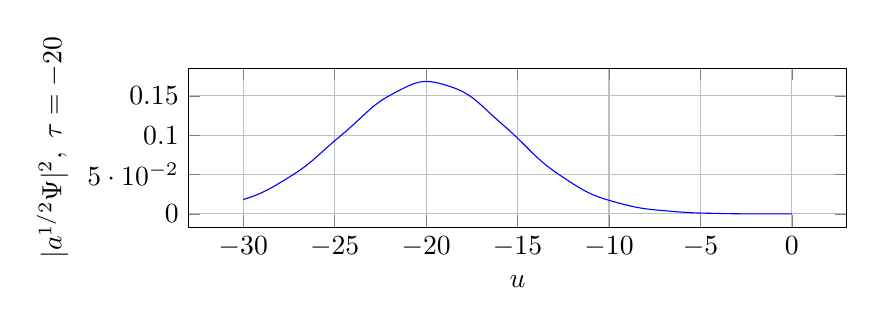
\begin{tikzpicture}
\begin{axis}[width=.82\textwidth,height=3.6cm,xlabel={$u$},ylabel={$|a^{1/2}\Psi|^2,\ \tau=-20$},grid=major,legend style={font=\small},]
\addplot+[mark=none] coordinates{(-30,0.0182853421) (-29.9,0.0190209096) (-29.8,0.0197727997) (-29.7,0.0205448324) (-29.6,0.0213413867) (-29.5,0.0221671574) (-29.4,0.0230268783) (-29.3,0.0239250329) (-29.2,0.0248655689) (-29.1,0.0258516376) (-29,0.0268853756) (-28.9,0.0279677462) (-28.8,0.0290984522) (-28.7,0.0302759291) (-28.6,0.0314974214) (-28.5,0.0327591398) (-28.4,0.0340564913) (-28.3,0.0353843696) (-28.2,0.0367374871) (-28.1,0.0381107283) (-28,0.039499502) (-27.9,0.0409000671) (-27.8,0.0423098108) (-27.7,0.0437274583) (-27.6,0.0451531978) (-27.5,0.04658871) (-27.4,0.0480370972) (-27.3,0.0495027135) (-27.2,0.0509909039) (-27.1,0.0525076673) (-27,0.054059264) (-26.9,0.0556517901) (-26.8,0.0572907479) (-26.7,0.0589806386) (-26.6,0.0607246068) (-26.5,0.0625241585) (-26.4,0.0643789763) (-26.3,0.0662868437) (-26.2,0.0682436881) (-26.1,0.0702437413) (-26,0.0722798114) (-25.9,0.0743436494) (-25.8,0.0764263911) (-25.7,0.0785190447) (-25.6,0.0806129963) (-25.5,0.0827004986) (-25.4,0.0847751123) (-25.3,0.0868320698) (-25.2,0.0888685362) (-25.1,0.090883749) (-25,0.0928790238) (-24.9,0.0948576239) (-24.8,0.0968244995) (-24.7,0.0987859097) (-24.6,0.10074895) (-24.5,0.102721016) (-24.4,0.104709227) (-24.3,0.106719867) (-24.2,0.108757847) (-24.1,0.110826261) (-24,0.112926027) (-23.9,0.115055678) (-23.8,0.117211278) (-23.7,0.119386504) (-23.6,0.121572874) (-23.5,0.12376011) (-23.4,0.125936625) (-23.3,0.12809009) (-23.2,0.130208067) (-23.1,0.132278643) (-23,0.134291051) (-22.9,0.136236222) (-22.8,0.138107239) (-22.7,0.139899664) (-22.6,0.141611713) (-22.5,0.143244271) (-22.4,0.144800737) (-22.3,0.146286715) (-22.2,0.147709572) (-22.1,0.149077871) (-22,0.150400737) (-21.9,0.151687176) (-21.8,0.15294541) (-21.7,0.15418224) (-21.6,0.155402507) (-21.5,0.156608671) (-21.4,0.157800532) (-21.3,0.158975121) (-21.2,0.160126759) (-21.1,0.161247294) (-21,0.16232649) (-20.9,0.163352549) (-20.8,0.16431274) (-20.7,0.165194093) (-20.6,0.165984107) (-20.5,0.166671448) (-20.4,0.167246578) (-20.3,0.16770228) (-20.2,0.168034054) (-20.1,0.168240351) (-20,0.168322634) (-19.9,0.168285268) (-19.8,0.168135231) (-19.7,0.167881683) (-19.6,0.167535407) (-19.5,0.167108154) (-19.4,0.166611946) (-19.3,0.166058363) (-19.2,0.165457869) (-19.1,0.164819214) (-19,0.164148942) (-18.9,0.163451048) (-18.8,0.162726788) (-18.7,0.161974661) (-18.6,0.161190569) (-18.5,0.160368127) (-18.4,0.159499117) (-18.3,0.15857406) (-18.2,0.157582854) (-18.1,0.156515455) (-18,0.155362559) (-17.9,0.154116227) (-17.8,0.152770441) (-17.7,0.151321536) (-17.6,0.149768503) (-17.5,0.148113126) (-17.4,0.146359963) (-17.3,0.144516171) (-17.2,0.142591172) (-17.1,0.14059621) (-17,0.138543795) (-16.9,0.136447093) (-16.8,0.134319285) (-16.7,0.132172938) (-16.6,0.13001942) (-16.5,0.127868404) (-16.4,0.125727467) (-16.3,0.123601834) (-16.2,0.121494249) (-16.1,0.119405003) (-16,0.117332101) (-15.9,0.115271552) (-15.8,0.113217778) (-15.7,0.111164098) (-15.6,0.109103269) (-15.5,0.107028041) (-15.4,0.104931709) (-15.3,0.102808609) (-15.2,0.100654547) (-15.1,0.0984671313) (-15,0.0962459901) (-14.9,0.0939928673) (-14.8,0.0917115911) (-14.7,0.0894079231) (-14.6,0.0870892974) (-14.5,0.0847644687) (-14.4,0.0824430908) (-14.3,0.0801352532) (-14.2,0.0778510008) (-14.1,0.0755998666) (-14,0.0733904424) (-13.9,0.0712300107) (-13.8,0.0691242566) (-13.7,0.0670770744) (-13.6,0.0650904748) (-13.5,0.0631645965) (-13.4,0.0612978175) (-13.3,0.0594869557) (-13.2,0.0577275455) (-13.1,0.0560141721) (-13,0.0543408426) (-12.9,0.0527013718) (-12.8,0.0510897613) (-12.7,0.0495005509) (-12.6,0.0479291234) (-12.5,0.0463719493) (-12.4,0.0448267574) (-12.3,0.0432926288) (-12.2,0.0417700083) (-12.1,0.0402606385) (-12,0.0387674229) (-11.9,0.0372942269) (-11.8,0.0358456329) (-11.7,0.0344266621) (-11.6,0.0330424817) (-11.5,0.0316981126) (-11.4,0.0303981546) (-11.3,0.0291465424) (-11.2,0.0279463449) (-11.1,0.0267996168) (-11,0.0257073084) (-10.9,0.024669235) (-10.8,0.0236841068) (-10.7,0.0227496139) (-10.6,0.0218625599) (-10.5,0.0210190353) (-10.4,0.0202146195) (-10.3,0.0194446002) (-10.2,0.0187041971) (-10.1,0.0179887795) (-10,0.0172940658) (-9.9,0.0166162948) (-9.8,0.0159523641) (-9.7,0.0152999258) (-9.6,0.0146574412) (-9.5,0.0140241893) (-9.4,0.0134002339) (-9.3,0.0127863522) (-9.2,0.0121839287) (-9.1,0.0115948246) (-9,0.0110212271) (-8.9,0.0104654904) (-8.8,0.00992997476) (-8.7,0.00941689279) (-8.6,0.00892817099) (-8.5,0.0084653321) (-8.4,0.00802940403) (-8.3,0.0076208586) (-8.2,0.00723958211) (-8.1,0.00688487775) (-8,0.00655549847) (-7.9,0.00624970736) (-7.8,0.00596536117) (-7.7,0.00570001184) (-7.6,0.00545102002) (-7.5,0.00521567422) (-7.4,0.00499130928) (-7.3,0.00477541802) (-7.2,0.00456575063) (-7.1,0.00436039708) (-7,0.00415784911) (-6.9,0.00395703926) (-6.8,0.003757356) (-6.7,0.00355863503) (-6.6,0.00336112833) (-6.5,0.00316545344) (-6.4,0.00297252645) (-6.3,0.00278348306) (-6.2,0.00259959229) (-6.1,0.00242216777) (-6,0.00225248157) (-5.9,0.00209168488) (-5.8,0.00194073967) (-5.7,0.00180036445) (-5.6,0.00167099643) (-5.5,0.00155277131) (-5.4,0.00144552105) (-5.3,0.00134878881) (-5.2,0.00126185936) (-5.1,0.0011838025) (-5,0.00111352635) (-4.9,0.00104983711) (-4.8,0.00099150134) (-4.7,0.000937307265) (-4.6,0.000886121564) (-4.5,0.000836938594) (-4.4,0.000788919661) (-4.3,0.000741420587) (-4.2,0.000694006651) (-4.1,0.000646454741) (-4,0.000598743373) (-3.9,0.000551031887) (-3.8,0.000503630731) (-3.7,0.000456965171) (-3.6,0.000411535025) (-3.5,0.000367873115) (-3.4,0.000326505031) (-3.3,0.000287912573) (-3.2,0.00025250283) (-3.1,0.000220584402) (-3,0.000192351672) (-2.9,0.000167877505) (-2.8,0.000147114136) (-2.7,0.000129901533) (-2.6,0.000115982047) (-2.5,0.000105019877) (-2.4,9.66236353e-05) (-2.3,9.03702538e-05) (-2.2,8.58285158e-05) (-2.1,8.25806686e-05) (-2,8.02408472e-05) (-1.9,7.84693719e-05) (-1.8,7.69823682e-05) (-1.7,7.555655e-05) (-1.6,7.40293781e-05) (-1.5,7.229514e-05) (-1.4,7.02977533e-05) (-1.3,6.80212759e-05) (-1.2,6.54791925e-05) (-1.1,6.27035406e-05) (-1,5.97348472e-05) (-0.9,5.6613684e-05) (-0.8,5.33744269e-05) (-0.7,5.00415533e-05) (-0.6,4.66285477e-05) (-0.5,4.31392302e-05) (-0.4,3.95711077e-05) (-0.3,3.59201759e-05) (-0.2,3.21864913e-05) (-0.1,2.83797932e-05) (0,2.45244837e-05)};
\end{axis}\end{tikzpicture}\end{center}
\begin{center}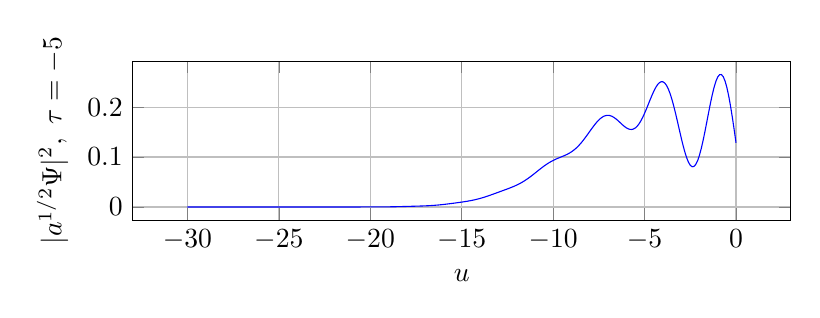
\begin{tikzpicture}
\begin{axis}[width=.82\textwidth,height=3.6cm,xlabel={$u$},ylabel={$|a^{1/2}\Psi|^2,\ \tau=-5$},grid=major,legend style={font=\small},]
\addplot+[mark=none] coordinates{(-30,1.09643614e-05) (-29.9,9.33919117e-06) (-29.8,7.58508438e-06) (-29.7,5.84841971e-06) (-29.6,4.276009e-06) (-29.5,3.00316797e-06) (-29.4,2.14258683e-06) (-29.3,1.77491419e-06) (-29.2,1.94183833e-06) (-29.1,2.64225515e-06) (-29,3.83186729e-06) (-28.9,5.42628376e-06) (-28.8,7.30740543e-06) (-28.7,9.33261254e-06) (-28.6,1.13460378e-05) (-28.5,1.31910319e-05) (-28.4,1.47228226e-05) (-28.3,1.5820343e-05) (-28.2,1.63962625e-05) (-28.1,1.64043902e-05) (-28,1.58438269e-05) (-27.9,1.47594997e-05) (-27.8,1.32390032e-05) (-27.7,1.14059705e-05) (-27.6,9.41048152e-06) (-27.5,7.41725833e-06) (-27.4,5.59258412e-06) (-27.3,4.09099225e-06) (-27.2,3.04279721e-06) (-27.1,2.54347888e-06) (-27,2.64578694e-06) (-26.9,3.35521723e-06) (-26.8,4.62924157e-06) (-26.7,6.38037074e-06) (-26.6,8.4828195e-06) (-26.5,1.078225e-05) (-26.4,1.31078184e-05) (-26.3,1.52855618e-05) (-26.2,1.71520498e-05) (-26.1,1.85672055e-05) (-26,1.94252649e-05) (-25.9,1.96629966e-05) (-25.8,1.92645279e-05) (-25.7,1.82624005e-05) (-25.6,1.67347867e-05) (-25.5,1.47991124e-05) (-25.4,1.26026244e-05) (-25.3,1.0310687e-05) (-25.2,8.09377297e-06) (-25.1,6.11421604e-06) (-25,4.51379815e-06) (-24.9,3.40316759e-06) (-24.8,2.85391887e-06) (-24.7,2.89393331e-06) (-24.6,3.50629769e-06) (-24.5,4.63181301e-06) (-24.4,6.17480193e-06) (-24.3,8.01164892e-06) (-24.2,1.00012852e-05) (-24.1,1.19966805e-05) (-24,1.385634e-05) (-23.9,1.54548273e-05) (-23.8,1.66914516e-05) (-23.7,1.74964448e-05) (-23.6,1.78342025e-05) (-23.5,1.77034532e-05) (-23.4,1.71345081e-05) (-23.3,1.61840248e-05) (-23.2,1.49279453e-05) (-23.1,1.34534342e-05) (-23,1.18507187e-05) (-22.9,1.02057227e-05) (-22.8,8.59427743e-06) (-22.7,7.07850517e-06) (-22.6,5.70571795e-06) (-22.5,4.50987836e-06) (-22.4,3.51536405e-06) (-22.3,2.74249152e-06) (-22.2,2.21402033e-06) (-22.1,1.96170171e-06) (-22,2.03187722e-06) (-21.9,2.48918418e-06) (-21.8,3.41758704e-06) (-21.7,4.91821695e-06) (-21.6,7.10384582e-06) (-21.5,1.00902149e-05) (-21.4,1.3984846e-05) (-21.3,1.88743421e-05) (-21.2,2.48114967e-05) (-21.1,3.18037332e-05) (-21,3.98044643e-05) (-20.9,4.87088704e-05) (-20.8,5.83553444e-05) (-20.7,6.85334436e-05) (-20.6,7.89986526e-05) (-20.5,8.9493635e-05) (-20.4,9.97749794e-05) (-20.3,0.000109643797) (-20.2,0.00011897795) (-20.1,0.000127763266) (-20,0.000136120835) (-19.9,0.000144327496) (-19.8,0.000152826866) (-19.7,0.000162228757) (-19.6,0.000173295605) (-19.5,0.000186915464) (-19.4,0.000204062218) (-19.3,0.000225744802) (-19.2,0.000252948345) (-19.1,0.000286571118) (-19,0.000327361928) (-18.9,0.000375863069) (-18.8,0.00043236397) (-18.7,0.000496870405) (-18.6,0.000569093311) (-18.5,0.000648460157) (-18.4,0.000734150258) (-18.3,0.000825153739) (-18.2,0.000920351929) (-18.1,0.00101861512) (-18,0.0011189119) (-17.9,0.00122042289) (-17.8,0.00132265068) (-17.7,0.00142551731) (-17.6,0.00152944105) (-17.5,0.00163538477) (-17.4,0.00174486994) (-17.3,0.0018599523) (-17.2,0.00198315783) (-17.1,0.00211738046) (-17,0.00226574599) (-16.9,0.00243144953) (-16.8,0.00261757636) (-16.7,0.00282691806) (-16.6,0.00306179704) (-16.5,0.00332391302) (-16.4,0.00361422439) (-16.3,0.00393287576) (-16.2,0.00427918052) (-16.1,0.00465166376) (-16,0.00504816697) (-15.9,0.00546601145) (-15.8,0.00590221279) (-15.7,0.00635373471) (-15.6,0.00681776651) (-15.5,0.00729200577) (-15.4,0.00777492615) (-15.3,0.00826600966) (-15.2,0.00876592394) (-15.1,0.0092766277) (-15,0.00980139125) (-14.9,0.0103447242) (-14.8,0.0109122087) (-14.7,0.0115102433) (-14.6,0.0121457077) (-14.5,0.0128255687) (-14.4,0.0135564482) (-14.3,0.0143441823) (-14.2,0.0151934027) (-14.1,0.0161071686) (-14,0.0170866822) (-13.9,0.0181311109) (-13.8,0.0192375388) (-13.7,0.0204010581) (-13.6,0.0216150079) (-13.5,0.022871352) (-13.4,0.0241611819) (-13.3,0.0254753208) (-13.2,0.0268049934) (-13.1,0.0281425237) (-13,0.0294820143) (-12.9,0.0308199614) (-12.8,0.0321557597) (-12.7,0.0334920552) (-12.6,0.0348349114) (-12.5,0.0361937638) (-12.4,0.0375811485) (-12.3,0.0390122063) (-12.2,0.0405039746) (-12.1,0.0420744967) (-12,0.0437417887) (-11.9,0.0455227173) (-11.8,0.0474318496) (-11.7,0.0494803422) (-11.6,0.0516749374) (-11.5,0.0540171346) (-11.4,0.0565025958) (-11.3,0.0591208367) (-11.2,0.06185524) (-11.1,0.0646834106) (-11,0.0675778773) (-10.9,0.0705071227) (-10.8,0.0734369061) (-10.7,0.0763318272) (-10.6,0.0791570595) (-10.5,0.0818801742) (-10.4,0.0844729619) (-10.3,0.0869131595) (-10.2,0.0891859872) (-10.1,0.0912854076) (-10,0.0932150276) (-9.9,0.0949885801) (-9.8,0.0966299376) (-9.7,0.0981726336) (-9.6,0.0996588875) (-9.5,0.101138153) (-9.4,0.102665232) (-9.3,0.104298023) (-9.2,0.106094977) (-9.1,0.108112368) (-9,0.11040149) (-8.9,0.113005889) (-8.8,0.115958759) (-8.7,0.11928062) (-8.6,0.122977382) (-8.5,0.12703891) (-8.4,0.131438157) (-8.3,0.136130943) (-8.2,0.141056429) (-8.1,0.146138288) (-8,0.151286588) (-7.9,0.156400347) (-7.8,0.161370696) (-7.7,0.166084588) (-7.6,0.17042892) (-7.5,0.174294966) (-7.4,0.177582947) (-7.3,0.180206598) (-7.2,0.182097542) (-7.1,0.183209304) (-7,0.183520766) (-6.9,0.183038903) (-6.8,0.181800632) (-6.7,0.179873625) (-6.6,0.177355973) (-6.5,0.17437462) (-6.4,0.171082508) (-6.3,0.167654462) (-6.2,0.164281842) (-6.1,0.161166085) (-6,0.158511301) (-5.9,0.156516142) (-5.8,0.155365207) (-5.7,0.155220312) (-5.6,0.15621198) (-5.5,0.158431508) (-5.4,0.161924033) (-5.3,0.166682951) (-5.2,0.172646062) (-5.1,0.179693753) (-5,0.187649475) (-4.9,0.196282684) (-4.8,0.205314322) (-4.7,0.214424815) (-4.6,0.223264435) (-4.5,0.231465758) (-4.4,0.238657838) (-4.3,0.24448159) (-4.2,0.2486058) (-4.1,0.250743089) (-4,0.250665111) (-3.9,0.248216253) (-3.8,0.243325116) (-3.7,0.236013092) (-3.6,0.226399471) (-3.5,0.214702603) (-3.4,0.201236805) (-3.3,0.186404878) (-3.2,0.170686304) (-3.1,0.15462138) (-3,0.138791772) (-2.9,0.123798161) (-2.8,0.110235816) (-2.7,0.0986690999) (-2.6,0.0896059918) (-2.5,0.083473796) (-2.4,0.0805971845) (-2.3,0.0811796952) (-2.2,0.0852896862) (-2.1,0.0928515956) (-2,0.103643142) (-1.9,0.117298858) (-1.8,0.133320067) (-1.7,0.151091111) (-1.6,0.169901363) (-1.5,0.18897223) (-1.4,0.207488117) (-1.3,0.224630107) (-1.2,0.2396109) (-1.1,0.251709497) (-1,0.260304044) (-0.9,0.264901282) (-0.8,0.265161201) (-0.7,0.260915621) (-0.6,0.252179727) (-0.5,0.239155832) (-0.4,0.222229044) (-0.3,0.201954817) (-0.2,0.179038799) (-0.1,0.154309725) (0,0.128686435)};
\end{axis}\end{tikzpicture}\end{center}
\begin{center}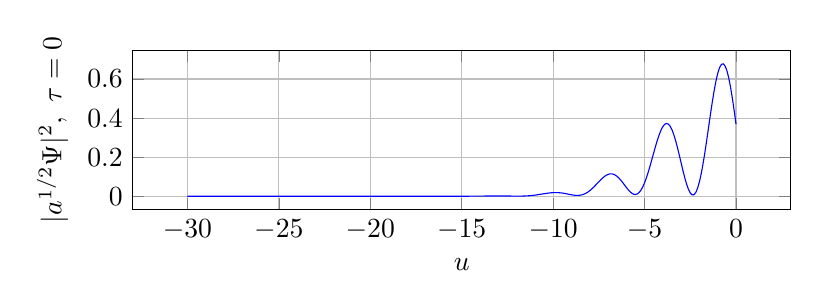
\begin{tikzpicture}
\begin{axis}[width=.82\textwidth,height=3.6cm,xlabel={$u$},ylabel={$|a^{1/2}\Psi|^2,\ \tau=0$},grid=major,legend style={font=\small},]
\addplot+[mark=none] coordinates{(-30,9.15017576e-06) (-29.9,7.65202078e-06) (-29.8,6.01762769e-06) (-29.7,4.38143068e-06) (-29.6,2.87944638e-06) (-29.5,1.63820695e-06) (-29.4,7.64346255e-07) (-29.3,3.3569485e-07) (-29.2,3.94625901e-07) (-29.1,9.4421904e-07) (-29,1.9475859e-06) (-28.9,3.33044723e-06) (-28.8,4.98678739e-06) (-28.7,6.78715938e-06) (-28.6,8.58899244e-06) (-28.5,1.02480838e-05) (-28.4,1.16303502e-05) (-28.3,1.26228837e-05) (-28.2,1.3143401e-05) (-28.1,1.31472977e-05) (-28,1.26317041e-05) (-27.9,1.16361782e-05) (-27.8,1.02399404e-05) (-27.7,8.55583758e-06) (-27.6,6.72149096e-06) (-27.5,4.88832062e-06) (-27.4,3.20931786e-06) (-27.3,1.8265511e-06) (-27.2,8.59423598e-07) (-27.1,3.94651541e-07) (-27,4.78802232e-07) (-26.9,1.11403226e-06) (-26.8,2.25741167e-06) (-26.7,3.82393129e-06) (-26.6,5.69299027e-06) (-26.5,7.71787369e-06) (-26.4,9.73747948e-06) (-26.3,1.15893611e-05) (-26.2,1.31230329e-05) (-26.1,1.42124518e-05) (-26,1.47666416e-05) (-25.9,1.47375679e-05) (-25.8,1.41245837e-05) (-25.7,1.29750395e-05) (-25.6,1.13809619e-05) (-25.5,9.47202366e-06) (-25.4,7.40533633e-06) (-25.3,5.35286489e-06) (-25.2,3.48746635e-06) (-25.1,1.96868218e-06) (-25,9.29448244e-07) (-24.9,4.6482557e-07) (-24.8,6.23704126e-07) (-24.7,1.40419988e-06) (-24.6,2.753172e-06) (-24.5,4.56995418e-06) (-24.4,6.71404976e-06) (-24.3,9.01621091e-06) (-24.2,1.12920369e-05) (-24.1,1.33570077e-05) (-24,1.50417357e-05) (-23.9,1.62061851e-05) (-23.8,1.67516735e-05) (-23.7,1.66296378e-05) (-23.6,1.58463961e-05) (-23.5,1.44634557e-05) (-23.4,1.25932761e-05) (-23.3,1.03907676e-05) (-23.2,8.04115959e-06) (-23.1,5.7451811e-06) (-23,3.70272886e-06) (-22.9,2.09634148e-06) (-22.8,1.07583332e-06) (-22.7,7.45368261e-07) (-22.6,1.15407314e-06) (-22.5,2.29101897e-06) (-22.4,4.08505381e-06) (-22.3,6.40958285e-06) (-22.2,9.09198922e-06) (-22.1,1.19270059e-05) (-22,1.46930164e-05) (-21.9,1.71700066e-05) (-21.8,1.91577367e-05) (-21.7,2.04926582e-05) (-21.6,2.10621825e-05) (-21.5,2.08150947e-05) (-21.4,1.97672002e-05) (-21.3,1.80016614e-05) (-21.2,1.56638971e-05) (-21.1,1.29513548e-05) (-21,1.0098879e-05) (-20.9,7.36076361e-06) (-20.8,4.99085581e-06) (-20.7,3.22225673e-06) (-20.6,2.24821746e-06) (-20.5,2.20575915e-06) (-20.4,3.16335275e-06) (-20.3,5.11369383e-06) (-20.2,7.97222315e-06) (-20.1,1.15816041e-05) (-20,1.57219081e-05) (-19.9,2.01258156e-05) (-19.8,2.44977459e-05) (-19.7,2.85355193e-05) (-19.6,3.19529492e-05) (-19.5,3.45016803e-05) (-19.4,3.59906383e-05) (-19.3,3.63016247e-05) (-19.2,3.53998825e-05) (-19.1,3.33388239e-05) (-19,3.02585519e-05) (-18.9,2.63782608e-05) (-18.8,2.19830525e-05) (-18.7,1.74061078e-05) (-18.6,1.30074779e-05) (-18.5,9.15099079e-06) (-18.4,6.18087792e-06) (-18.3,4.39971378e-06) (-18.2,4.0491338e-06) (-18.1,5.29455809e-06) (-18,8.2148296e-06) (-17.9,1.27972983e-05) (-17.8,1.89384814e-05) (-17.7,2.64500364e-05) (-17.6,3.50694296e-05) (-17.5,4.44743946e-05) (-17.4,5.43000755e-05) (-17.3,6.41576488e-05) (-17.2,7.36532197e-05) (-17.1,8.240589e-05) (-17,9.00640781e-05) (-16.9,9.63194203e-05) (-16.8,0.000100917865) (-16.7,0.000103667864) (-16.6,0.000104445846) (-16.5,0.000103199372) (-16.4,9.99485357e-05) (-16.3,9.47862787e-05) (-16.2,8.78782313e-05) (-16.1,7.94626512e-05) (-16,6.98508296e-05) (-15.9,5.94281213e-05) (-15.8,4.86554885e-05) (-15.7,3.80711718e-05) (-15.6,2.82918424e-05) (-15.5,2.00123664e-05) (-15.4,1.40031551e-05) (-15.3,1.11039947e-05) (-15.2,1.22132598e-05) (-15.1,1.82715239e-05) (-15,3.02387818e-05) (-14.9,4.90647935e-05) (-14.8,7.5652426e-05) (-14.7,0.000110814311) (-14.6,0.000155223617) (-14.5,0.000209360253) (-14.4,0.000273454354) (-14.3,0.000347429443) (-14.2,0.00043084815) (-14.1,0.000522863883) (-14,0.00062218224) (-13.9,0.000727036286) (-13.8,0.000835180047) (-13.7,0.000943904625) (-13.6,0.00105008119) (-13.5,0.00115023476) (-13.4,0.0012406519) (-13.3,0.00131752457) (-13.2,0.00137713078) (-13.1,0.00141605107) (-13,0.00143141725) (-12.9,0.00142118778) (-12.8,0.00138444055) (-12.7,0.00132167125) (-12.6,0.00123508225) (-12.5,0.00112884362) (-12.4,0.00100930598) (-12.3,0.000885142487) (-12.2,0.000767396933) (-12.1,0.000669415132) (-12,0.000606639078) (-11.9,0.000596247145) (-11.8,0.000656629438) (-11.7,0.000806695149) (-11.6,0.00106501829) (-11.5,0.00144883932) (-11.4,0.00197295227) (-11.3,0.00264851982) (-11.2,0.00348187114) (-11.1,0.00447334867) (-11,0.0056162794) (-10.9,0.00689615236) (-10.8,0.00829008638) (-10.7,0.00976666966) (-10.6,0.0112862445) (-10.5,0.012801697) (-10.4,0.0142597905) (-10.3,0.0156030578) (-10.2,0.0167722347) (-10.1,0.0177091841) (-10,0.0183602224) (-9.9,0.0186797236) (-9.8,0.0186338412) (-9.7,0.018204156) (-9.6,0.0173910358) (-9.5,0.0162164766) (-9.4,0.0147261936) (-9.3,0.012990737) (-9.2,0.0111054366) (-9.1,0.00918901499) (-9,0.00738076372) (-8.9,0.00583624556) (-8.8,0.00472156115) (-8.7,0.00420630561) (-8.6,0.00445542895) (-8.5,0.00562030168) (-8.4,0.00782936822) (-8.3,0.0111788401) (-8.2,0.0157239322) (-8.1,0.0214711751) (-8,0.0283723392) (-7.9,0.0363204795) (-7.8,0.0451485527) (-7.7,0.054630967) (-7.6,0.0644883074) (-7.5,0.0743953352) (-7.4,0.0839921911) (-7.3,0.0928985579) (-7.2,0.100730351) (-7.1,0.10711833) (-7,0.11172786) (-6.9,0.114278913) (-6.8,0.114565314) (-6.7,0.112472152) (-6.6,0.1079903) (-6.5,0.101227036) (-6.4,0.0924118484) (-6.3,0.0818967148) (-6.2,0.0701503278) (-6.1,0.0577460434) (-6,0.0453436125) (-5.9,0.033665087) (-5.8,0.0234656268) (-5.7,0.0155002496) (-5.6,0.0104878585) (-5.5,0.0090741254) (-5.4,0.0117949871) (-5.3,0.0190426126) (-5.2,0.0310357146) (-5.1,0.0477959931) (-5,0.0691323186) (-4.9,0.0946339873) (-4.8,0.123674015) (-4.7,0.155422999) (-4.6,0.188873591) (-4.5,0.222875076) (-4.4,0.256177054) (-4.3,0.287480658) (-4.2,0.315495318) (-4.1,0.338998643) (-4,0.356896735) (-3.9,0.368282032) (-3.8,0.372485767) (-3.7,0.36912221) (-3.6,0.358122115) (-3.5,0.339753194) (-3.4,0.314625937) (-3.3,0.283683757) (-3.2,0.248177125) (-3.1,0.209622139) (-3,0.169744737) (-2.9,0.130412535) (-2.8,0.0935569313) (-2.7,0.0610887412) (-2.6,0.034811047) (-2.5,0.0163332654) (-2.4,0.00699052048) (-2.3,0.00777233197) (-2.2,0.0192643291) (-2.1,0.0416062221) (-2,0.0744685992) (-1.9,0.117050313) (-1.8,0.168097293) (-1.7,0.225942629) (-1.6,0.288566758) (-1.5,0.35367558) (-1.4,0.418793421) (-1.3,0.481366967) (-1.2,0.538875656) (-1.1,0.588943593) (-1,0.629447837) (-0.9,0.658617991) (-0.8,0.675122251) (-0.7,0.678135668) (-0.6,0.667387063) (-0.5,0.64318201) (-0.4,0.606400339) (-0.3,0.558467822) (-0.2,0.50130287) (-0.1,0.437240278) (0,0.368935175)};
\end{axis}\end{tikzpicture}\end{center}
\begin{center}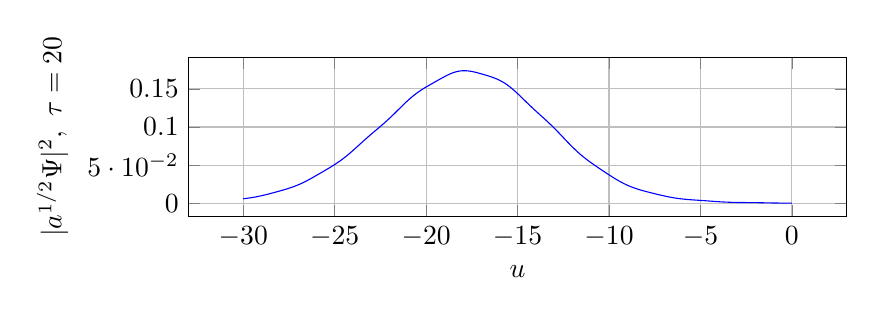
\begin{tikzpicture}
\begin{axis}[width=.82\textwidth,height=3.6cm,xlabel={$u$},ylabel={$|a^{1/2}\Psi|^2,\ \tau=20$},grid=major,legend style={font=\small},]
\addplot+[mark=none] coordinates{(-30,0.00577993229) (-29.9,0.00606391106) (-29.8,0.00636764878) (-29.7,0.00669435846) (-29.6,0.00704688913) (-29.5,0.00742754422) (-29.4,0.00783792951) (-29.3,0.00827884254) (-29.2,0.00875021343) (-29.1,0.00925110346) (-29,0.00977976437) (-28.9,0.010333757) (-28.8,0.0109101239) (-28.7,0.0115056061) (-28.6,0.0121168912) (-28.5,0.0127408772) (-28.4,0.0133749339) (-28.3,0.0140171441) (-28.2,0.0146665074) (-28.1,0.0153230892) (-28,0.0159881047) (-27.9,0.0166639267) (-27.8,0.0173540156) (-27.7,0.0180627708) (-27.6,0.0187953122) (-27.5,0.019557202) (-27.4,0.0203541249) (-27.3,0.0211915446) (-27.2,0.0220743611) (-27.1,0.0230065902) (-27,0.0239910885) (-26.9,0.0250293439) (-26.8,0.026121349) (-26.7,0.0272655676) (-26.6,0.0284590015) (-26.5,0.0296973556) (-26.4,0.0309752948) (-26.3,0.0322867782) (-26.2,0.0336254511) (-26.1,0.0349850702) (-26,0.0363599355) (-25.9,0.0377452995) (-25.8,0.0391377257) (-25.7,0.0405353705) (-25.6,0.0419381673) (-25.5,0.0433478975) (-25.4,0.044768138) (-25.3,0.0462040869) (-25.2,0.0476622731) (-25.1,0.0491501655) (-25,0.0506757043) (-24.9,0.0522467833) (-24.8,0.0538707142) (-24.7,0.0555537092) (-24.6,0.0573004151) (-24.5,0.0591135311) (-24.4,0.0609935388) (-24.3,0.0629385632) (-24.2,0.0649443804) (-24.1,0.0670045725) (-24,0.0691108263) (-23.9,0.071253359) (-23.8,0.0734214462) (-23.7,0.0756040228) (-23.6,0.0777903164) (-23.5,0.0799704767) (-23.4,0.0821361565) (-23.3,0.0842810084) (-23.2,0.086401061) (-23.1,0.0884949485) (-23,0.0905639747) (-22.9,0.0926120042) (-22.8,0.0946451826) (-22.7,0.0966715012) (-22.6,0.0987002295) (-22.5,0.100741249) (-22.4,0.102804332) (-22.3,0.104898404) (-22.2,0.107030843) (-22.1,0.109206857) (-22,0.111428989) (-21.9,0.113696767) (-21.8,0.116006543) (-21.7,0.118351525) (-21.6,0.120722004) (-21.5,0.123105769) (-21.4,0.12548868) (-21.3,0.12785538) (-21.2,0.130190086) (-21.1,0.132477417) (-21,0.134703224) (-20.9,0.136855332) (-20.8,0.138924195) (-20.7,0.140903374) (-20.6,0.142789842) (-20.5,0.144584076) (-20.4,0.146289931) (-20.3,0.147914305) (-20.2,0.149466612) (-20.1,0.150958087) (-20,0.152400984) (-19.9,0.153807685) (-19.8,0.155189811) (-19.7,0.156557363) (-19.6,0.157917955) (-19.5,0.1592762) (-19.4,0.160633267) (-19.3,0.161986655) (-19.2,0.163330197) (-19.1,0.164654292) (-19,0.165946347) (-18.9,0.167191426) (-18.8,0.168373032) (-18.7,0.169474016) (-18.6,0.170477517) (-18.5,0.171367909) (-18.4,0.172131677) (-18.3,0.172758172) (-18.2,0.173240209) (-18.1,0.173574452) (-18,0.173761581) (-17.9,0.173806216) (-17.8,0.173716614) (-17.7,0.173504147) (-17.6,0.1731826) (-17.5,0.172767331) (-17.4,0.17227434) (-17.3,0.17171931) (-17.2,0.17111667) (-17.1,0.170478752) (-17,0.169815071) (-16.9,0.169131792) (-16.8,0.168431408) (-16.7,0.167712639) (-16.6,0.166970572) (-16.5,0.166197024) (-16.4,0.165381105) (-16.3,0.164509945) (-16.2,0.163569548) (-16.1,0.162545706) (-16,0.161424934) (-15.9,0.160195356) (-15.8,0.158847495) (-15.7,0.15737492) (-15.6,0.155774715) (-15.5,0.154047732) (-15.4,0.152198634) (-15.3,0.150235707) (-15.2,0.148170467) (-15.1,0.146017093) (-15,0.143791695) (-14.9,0.141511504) (-14.8,0.139193991) (-14.7,0.136855994) (-14.6,0.134512902) (-14.5,0.132177929) (-14.4,0.129861539) (-14.3,0.127571032) (-14.2,0.125310331) (-14.1,0.123079972) (-14,0.120877284) (-13.9,0.118696762) (-13.8,0.116530596) (-13.7,0.114369317) (-13.6,0.112202535) (-13.5,0.110019711) (-13.4,0.107810914) (-13.3,0.105567535) (-13.2,0.103282898) (-13.1,0.100952747) (-13,0.0985755795) (-12.9,0.0961528088) (-12.8,0.0936887513) (-12.7,0.0911904447) (-12.6,0.088667311) (-12.5,0.086130687) (-12.4,0.0835932541) (-12.3,0.0810684032) (-12.2,0.0785695712) (-12.1,0.0761095914) (-12,0.0737000902) (-11.9,0.0713509679) (-11.8,0.0690699867) (-11.7,0.0668624888) (-11.6,0.0647312546) (-11.5,0.0626765049) (-11.4,0.0606960433) (-11.3,0.0587855228) (-11.2,0.0569388206) (-11.1,0.0551484933) (-11,0.0534062847) (-10.9,0.0517036558) (-10.8,0.0500323061) (-10.7,0.0483846568) (-10.6,0.0467542707) (-10.5,0.0451361882) (-10.4,0.0435271629) (-10.3,0.0419257895) (-10.2,0.0403325197) (-10.1,0.0387495717) (-10,0.0371807419) (-9.9,0.0356311344) (-9.8,0.0341068267) (-9.7,0.0326144926) (-9.6,0.0311610064) (-9.5,0.0297530499) (-9.4,0.0283967442) (-9.3,0.0270973255) (-9.2,0.025858881) (-9.1,0.0246841552) (-9,0.0235744351) (-8.9,0.0225295166) (-8.8,0.0215477497) (-8.7,0.0206261558) (-8.6,0.019760609) (-8.5,0.0189460671) (-8.4,0.0181768382) (-8.3,0.0174468671) (-8.2,0.0167500264) (-8.1,0.0160803948) (-8,0.0154325111) (-7.9,0.0148015911) (-7.8,0.014183698) (-7.7,0.0135758604) (-7.6,0.0129761347) (-7.5,0.0123836115) (-7.4,0.0117983691) (-7.3,0.0112213789) (-7.2,0.01065437) (-7.1,0.0100996633) (-7,0.00955998263) (-6.9,0.00903825659) (-6.8,0.00853741916) (-6.7,0.00806022049) (-6.6,0.00760905635) (-6.5,0.007185824) (-6.4,0.00679181033) (-6.3,0.00642761634) (-6.2,0.00609312008) (-6.1,0.00578747821) (-6,0.00550916424) (-5.9,0.00525604032) (-5.8,0.00502545737) (-5.7,0.00481437778) (-5.6,0.00461951351) (-5.5,0.00443747257) (-5.4,0.00426490608) (-5.3,0.00409864896) (-5.2,0.00393584747) (-5.1,0.00377406781) (-5,0.00361138111) (-4.9,0.00344642155) (-4.8,0.00327841538) (-4.7,0.00310718055) (-4.6,0.00293309781) (-4.5,0.00275705565) (-4.4,0.00258037249) (-4.3,0.00240470091) (-4.2,0.00223191901) (-4.1,0.002064015) (-4,0.00190297072) (-3.9,0.00175065033) (-3.8,0.00160869936) (-3.7,0.00147845907) (-3.6,0.0013608999) (-3.5,0.0012565768) (-3.4,0.00116560794) (-3.3,0.00108767703) (-3.2,0.00102205821) (-3.1,0.000967661409) (-3,0.000923094777) (-2.9,0.000886740324) (-2.8,0.000856838034) (-2.7,0.000831573592) (-2.6,0.000809164811) (-2.5,0.000787942098) (-2.4,0.000766418868) (-2.3,0.000743348539) (-2.2,0.000717765666) (-2.1,0.000689009825) (-2,0.000656731886) (-1.9,0.000620883403) (-1.8,0.000581690785) (-1.7,0.000539616725) (-1.6,0.000495311976) (-1.5,0.000449560987) (-1.4,0.000403225012) (-1.3,0.000357186273) (-1.2,0.00031229641) (-1.1,0.00026933194) (-1,0.000228958833) (-0.9,0.000191707497) (-0.8,0.000157958726) (-0.7,0.000127940345) (-0.6,0.000101733612) (-0.5,7.92878216e-05) (-0.4,6.04411494e-05) (-0.3,4.49455068e-05) (-0.2,3.24931212e-05) (-0.1,2.27426709e-05) (0,1.53430863e-05)};
\end{axis}\end{tikzpicture}\end{center}

\end{solution}
\originalsection{第5题：矩形障壁的三个能区}
\begin{exercise}
按MIT原件的矩形障壁任务, 势高$V_0>0$, 宽度未指定, 本处记为任意$d>0$, 障壁外势0. 求$E<V_0$、$E=V_0$透射率并问低于障壁能否$T=1$; 再独立求$E>V_0$及完全透射条件. 原件署Based on Griffiths 2.33.
\end{exercise}
\begin{solution}
取障壁区间$[0,d]$, 两侧波数$k=\sqrt{2mE}/\hbar$. 在$E<V_0$内写$Ae^{\kappa x}+Be^{-\kappa x}$, $\kappa=\sqrt{2m(V_0-E)}/\hbar$. 将连续的$\psi,\psi'$从0传播到$d$, 传播矩阵为$\left(\begin{smallmatrix}\cosh\kappa d&\sinh\kappa d/\kappa\\\kappa\sinh\kappa d&\cosh\kappa d\end{smallmatrix}\right)$. 代入左边$(1+r,\ii k(1-r))$及右边$t\e^{\ii kd}(1,\ii k)$, 消去$r$, 得$1/T=1+(k^2+\kappa^2)^2\sinh^2(\kappa d)/(4k^2\kappa^2)$. 因两外区相同, $T=|t|^2$, 故
\[
T=\left[1+\frac{V_0^2\sinh^2(\kappa d)}{4E(V_0-E)}\right]^{-1}<1.
\]
$E\to V_0$时$\sinh\kappa d\sim\kappa d$, 得$T=[1+mV_0d^2/(2\hbar^2)]^{-1}$. 高于障壁时内波数$q=\sqrt{2m(E-V_0)}/\hbar$, 传播矩阵以$\cos qd,\sin qd/q,-q\sin qd$替换, 得$T=[1+V_0^2\sin^2(qd)/(4E(E-V_0))]^{-1}$. $T=1$要求$qd=n\pi$, $n\ge1$, 是两接口多重反射的相消条件; $E=V_0$不能把$q=0$误计成共振.
\end{solution}
